% \documentclass[a5paper]{report}
% \usepackage[margin=40pt]{geometry}
% \documentclass{report}
\documentclass{book}

\usepackage[paperwidth=5.7in, paperheight=8.55in, margin=1.25cm]{geometry}
\setlength{\footskip}{\dimexpr\footskip-.3cm\relax}

\usepackage{hyperref}
\usepackage{fontspec}
\usepackage{dsfont}
\usepackage{microtype}
\usepackage[english]{babel}
\usepackage[T1]{fontenc}
\usepackage{graphicx} 
\usepackage{wrapfig}
\usepackage{enumitem}
\usepackage{anyfontsize}
\usepackage{amsmath,amssymb}
\usepackage{tikz,tikz-layers}
\usetikzlibrary{calc,positioning,fit}

% strenghts and weakness colors
\definecolor{mygreen}{HTML}{edf7ec}
\definecolor{myred}{HTML}{fbecec}

% chapters colors
\definecolor{cyanlight}{HTML}{d3f9ff}
\definecolor{purplelight}{HTML}{b7a1d0}
\definecolor{orangelight}{HTML}{ffecc6}
\definecolor{corallight}{HTML}{FFDEDE}
\definecolor{mintlight}{HTML}{CAFFC4}

\definecolor{cyanhard}{HTML}{9CF2FF}
\definecolor{purplehard}{HTML}{A97ADE}
\definecolor{orangehard}{HTML}{FFD689}
\definecolor{coralhard}{HTML}{FFA5A5}
\definecolor{minthard}{HTML}{A1FF98}

% formula colors
\definecolor{nmlpurple}{HTML}{3B0280}
\definecolor{nmlcyan}{HTML}{00C8E5}
\definecolor{nmlred}{HTML}{DD4040}
\definecolor{nmlgreen}{HTML}{4EB046}
\definecolor{nmlyellow}{HTML}{E1BC29}



\setsansfont{Lato}[
    Path=./fonts/LatoFont/,
    % Scale=0.9,
    Extension = .ttf,
    UprightFont=*-Regular,
    BoldFont=*-Bold,
    ItalicFont=*-Italic,
    BoldItalicFont=*-BoldItalic
    ]

\setmainfont{Rubik}[
    Path=./fonts/RubikFont/,
    % Scale=0.9,
    Extension = .ttf,
    UprightFont=*-Regular,
    BoldFont=*-SemiBold,
    ItalicFont=*-Italic,
    BoldItalicFont=*-BoldItalic
    ]

\setmonofont{PlayfairDisplay}[
    Path=./fonts/PlayFairFont/,
    % Scale=0.85,
    Extension = .ttf,
    UprightFont=*-Regular,
    BoldFont=*-Bold,
    ItalicFont=*-Italic,
    BoldItalicFont=*-BoldItalic
    ]

%============================================================================
\usepackage{fancyhdr}

% Redefine \section to center the title without number
\makeatletter
\renewcommand\section{\@startsection{section}{1}{\z@}%
  {-3.5ex \@plus -1ex \@minus -.2ex}%
  {0.3ex \@plus.2ex}%
  {\Large\bfseries\centering}}
\makeatother

% Redefine \subsection to center the title without number
\makeatletter
\renewcommand\subsection{\@startsection{subsection}{2}{\z@}%
  {-0.25ex\@plus -1ex \@minus -.2ex}%
  {1.5ex \@plus .2ex}%
  {\large\centering}}
\makeatother

% Remove visible section numbering but keep it in the .aux file for references
\setcounter{secnumdepth}{0}

% Define commands to store chapter, section title and number
\newcommand{\chaptertitle}{}
\newcommand{\sectiontitle}{}

% New command for chapters
\renewcommand{\chapter}[1]{%
    \refstepcounter{chapter}% Increment the chapter counter
    \clearpage
    \thispagestyle{empty}
    \vspace*{\fill}
    {\centering\huge\bfseries #1\par}
    \vspace*{\fill}
    \clearpage
    \renewcommand{\chaptertitle}{#1}%
}

% Redefine \section to update the mark and store the title
\let\oldsection\section
\renewcommand{\section}[1]{%
    \refstepcounter{section}% Increment the section counter
    \oldsection{#1}%
    \markboth{#1}{#1}% Store only title in both marks
    \renewcommand{\sectiontitle}{#1}% Store the title for use in the style
}

\fancypagestyle{regressionstyle}{
    \fancyhf{} % Clear all header and footer fields
    \fancyfoot[L]{\color{black!40}Daily metrics at nannyml.com/metrics} % Bottom left
    \fancyfoot[R]{\thesection\ \chaptertitle: \sectiontitle} % Bottom right, includes chapter.section number, chapter title, and section title
    \renewcommand{\headrulewidth}{0pt} % Remove header line
    \renewcommand{\footrulewidth}{0pt} % Remove footer line if undesired
    \tikz[overlay,remember picture]
    {
    \node[inner sep=0pt,outer sep=0pt,minimum width=.7cm, minimum height=\paperheight, anchor=north west, fill=cyanlight] (a) at (current page.north west) {};
    \node[anchor=east, rotate=90, xshift=-.5cm] at (a.north) 
    {
    \chaptertitle\ -- \sectiontitle % Chapter and section title here
    }; 
    }
}


\fancypagestyle{classificationstyle}{
    \fancyhf{} % Clear all header and footer fields
    \fancyfoot[L]{\color{black!40}Daily metrics at nannyml.com/metrics} % Bottom left
    \fancyfoot[R]{\thesection\ \chaptertitle: \sectiontitle} % Bottom right, includes chapter.section number, chapter title, and section title
    \renewcommand{\headrulewidth}{0pt} % Remove header line
    % \renewcommand{\fchapters colorsootrulewidth}{0pt} % Remove footer line if undesired
    \tikz[overlay,remember picture]
    {
    \node[inner sep=0pt,outer sep=0pt,minimum width=.7cm, minimum height=\paperheight, anchor=north west, fill=purplelight] (a) at (current page.north west) {};
    \node[anchor=east, rotate=90, xshift=-.5cm] at (a.north) 
    {
    \chaptertitle\ -- \sectiontitle % Chapter and section title here
    }; 
    }
}

\fancypagestyle{clusteringstyle}{
    \fancyhf{} % Clear all header and footer fields
    \fancyfoot[L]{\color{black!40}Daily metrics at nannyml.com/metrics} % Bottom left
    \fancyfoot[R]{\thesection\ \chaptertitle: \sectiontitle} % Bottom right, includes chapter.section number, chapter title, and section title
    \renewcommand{\headrulewidth}{0pt} % Remove header line
    % \renewcommand{\fchapters colorsootrulewidth}{0pt} % Remove footer line if undesired
    \tikz[overlay,remember picture]
    {
    \node[inner sep=0pt,outer sep=0pt,minimum width=.7cm, minimum height=\paperheight, anchor=north west, fill=orangelight] (a) at (current page.north west) {};
    \node[anchor=east, rotate=90, xshift=-.5cm] at (a.north) 
    {
    \chaptertitle\ -- \sectiontitle % Chapter and section title here
    }; 
    }
}

\fancypagestyle{rankingstyle}{
    \fancyhf{} % Clear all header and footer fields
    \fancyfoot[L]{\color{black!40}Daily metrics at nannyml.com/metrics} % Bottom left
    \fancyfoot[R]{\thesection\ \chaptertitle: \sectiontitle} % Bottom right, includes chapter.section number, chapter title, and section title
    \renewcommand{\headrulewidth}{0pt} % Remove header line
    % \renewcommand{\fchapters colorsootrulewidth}{0pt} % Remove footer line if undesired
    \tikz[overlay,remember picture]
    {
    \node[inner sep=0pt,outer sep=0pt,minimum width=.7cm, minimum height=\paperheight, anchor=north west, fill=corallight] (a) at (current page.north west) {};
    \node[anchor=east, rotate=90, xshift=-.5cm] at (a.north) 
    {
    \chaptertitle\ -- \sectiontitle % Chapter and section title here
    }; 
    }
}

\fancypagestyle{cvstyle}{
    \fancyhf{} % Clear all header and footer fields
    \fancyfoot[L]{\color{black!40}Daily metrics at nannyml.com/metrics} % Bottom left
    \fancyfoot[R]{\thesection\ \chaptertitle: \sectiontitle} % Bottom right, includes chapter.section number, chapter title, and section title
    \renewcommand{\headrulewidth}{0pt} % Remove header line
    % \renewcommand{\fchapters colorsootrulewidth}{0pt} % Remove footer line if undesired
    \tikz[overlay,remember picture]
    {
    \node[inner sep=0pt,outer sep=0pt,minimum width=.7cm, minimum height=\paperheight, anchor=north west, fill=mintlight] (a) at (current page.north west) {};
    \node[anchor=east, rotate=90, xshift=-.5cm] at (a.north) 
    {
    \chaptertitle\ -- \sectiontitle % Chapter and section title here
    }; 
    }
}

\fancypagestyle{nlpstyle}{
    \fancyhf{} % Clear all header and footer fields
    \fancyfoot[L]{\color{black!40}Daily metrics at nannyml.com/metrics} % Bottom left
    \fancyfoot[R]{\thesection\ \chaptertitle: \sectiontitle} % Bottom right, includes chapter.section number, chapter title, and section title
    \renewcommand{\headrulewidth}{0pt} % Remove header line
    % \renewcommand{\fchapters colorsootrulewidth}{0pt} % Remove footer line if undesired
    \tikz[overlay,remember picture]
    {
    \node[inner sep=0pt,outer sep=0pt,minimum width=.7cm, minimum height=\paperheight, anchor=north west, fill=cyanhard] (a) at (current page.north west) {};
    \node[anchor=east, rotate=90, xshift=-.5cm] at (a.north) 
    {
    \chaptertitle\ -- \sectiontitle % Chapter and section title here
    }; 
    }
}

\fancypagestyle{genaistyle}{
    \fancyhf{} % Clear all header and footer fields
    \fancyfoot[L]{\color{black!40}Daily metrics at nannyml.com/metrics} % Bottom left
    \fancyfoot[R]{\thesection\ \chaptertitle: \sectiontitle} % Bottom right, includes chapter.section number, chapter title, and section title
    \renewcommand{\headrulewidth}{0pt} % Remove header line
    % \renewcommand{\fchapters colorsootrulewidth}{0pt} % Remove footer line if undesired
    \tikz[overlay,remember picture]
    {
    \node[inner sep=0pt,outer sep=0pt,minimum width=.7cm, minimum height=\paperheight, anchor=north west, fill=purplehard] (a) at (current page.north west) {};
    \node[anchor=east, rotate=90, xshift=-.5cm] at (a.north) 
    {
    \chaptertitle\ -- \sectiontitle % Chapter and section title here
    }; 
    }
}

\fancypagestyle{probabilisticstyle}{
    \fancyhf{} % Clear all header and footer fields
    \fancyfoot[L]{\color{black!40}Daily metrics at nannyml.com/metrics} % Bottom left
    \fancyfoot[R]{\thesection\ \chaptertitle: \sectiontitle} % Bottom right, includes chapter.section number, chapter title, and section title
    \renewcommand{\headrulewidth}{0pt} % Remove header line
    % \renewcommand{\fchapters colorsootrulewidth}{0pt} % Remove footer line if undesired
    \tikz[overlay,remember picture]
    {
    \node[inner sep=0pt,outer sep=0pt,minimum width=.7cm, minimum height=\paperheight, anchor=north west, fill=orangehard] (a) at (current page.north west) {};
    \node[anchor=east, rotate=90, xshift=-.5cm] at (a.north) 
    {
    \chaptertitle\ -- \sectiontitle % Chapter and section title here
    }; 
    }
}

\fancypagestyle{biasfairnesstyle}{
    \fancyhf{} % Clear all header and footer fields
    \fancyfoot[L]{\color{black!40}Daily metrics at nannyml.com/metrics} % Bottom left
    \fancyfoot[R]{\thesection\ \chaptertitle: \sectiontitle} % Bottom right, includes chapter.section number, chapter title, and section title
    \renewcommand{\headrulewidth}{0pt} % Remove header line
    % \renewcommand{\fchapters colorsootrulewidth}{0pt} % Remove footer line if undesired
    \tikz[overlay,remember picture]
    {
    \node[inner sep=0pt,outer sep=0pt,minimum width=.7cm, minimum height=\paperheight, anchor=north west, fill=coralhard] (a) at (current page.north west) {};
    \node[anchor=east, rotate=90, xshift=-.5cm] at (a.north) 
    {
    \chaptertitle\ -- \sectiontitle % Chapter and section title here
    }; 
    }
}

\fancypagestyle{businessstyle}{
    \fancyhf{} % Clear all header and footer fields
    \fancyfoot[L]{\color{black!40}Daily metrics at nannyml.com/metrics} % Bottom left
    \fancyfoot[R]{\thesection\ \chaptertitle: \sectiontitle} % Bottom right, includes chapter.section number, chapter title, and section title
    \renewcommand{\headrulewidth}{0pt} % Remove header line
    % \renewcommand{\fchapters colorsootrulewidth}{0pt} % Remove footer line if undesired
    \tikz[overlay,remember picture]
    {
    \node[inner sep=0pt,outer sep=0pt,minimum width=.7cm, minimum height=\paperheight, anchor=north west, fill=minthard] (a) at (current page.north west) {};
    \node[anchor=east, rotate=90, xshift=-.5cm] at (a.north) 
    {
    \chaptertitle\ -- \sectiontitle % Chapter and section title here
    }; 
    }
}

\fancypagestyle{customstyle}{
    \fancyhf{} % Clear all header and footer fields
    \fancyfoot[L]{\color{black!40}Daily metrics at nannyml.com/metrics} % Bottom left
    \fancyfoot[R]{\thesection\ \chaptertitle: \sectiontitle} % Bottom right, includes chapter.section number, chapter title, and section title
    \renewcommand{\headrulewidth}{0pt} % Remove header line
    \renewcommand{\footrulewidth}{0pt} % Remove footer line if undesired
}

%============================================================================



\setlength{\parindent}{0pt}
\setlength{\parskip}{8pt}


\newcommand{\coloredboxes}[2]{
\tikz[every node/.style={outer sep=0pt, inner sep=0pt, align=left}] {
\node[ minimum width=.5\textwidth, minimum height=1cm, label={[yshift=-7.5mm]above:\strut\textbf{Strength}}] (a) {
\\[.7cm]
\parbox{.45\textwidth}{
\begin{itemize}[left=0pt, label={\textcolor{teal!60!green!60}{$\bullet$}}]
    #1
\end{itemize}
}

};

\path let \p1 = (a.north), \p2 = (a.south) in
node[ minimum width=.5\textwidth, minimum height=\y1-\y2, 
label={[yshift=-7.5mm]above:\strut\textbf{Weakness}}, anchor=north west] (b) at (a.north east) {
\\[.7cm]
\parbox{.45\textwidth}{
\begin{itemize}[left=0pt, label={\textcolor{red!80!black!60}{$\bullet$}}]
    #2
\end{itemize}
}

};

\begin{scope}[on behind layer]
\fill[mygreen] (current bounding box.north)--($(current bounding box.north west)+(.4,0)$) to[bend right=45] ($(current bounding box.north west)+(0,-.4)$)--($(current bounding box.south west)+(0,.4)$) to[bend right=45] ($(current bounding box.south west)+(.4,0)$)--(current bounding box.south)--cycle;    
\end{scope}

\begin{scope}[on behind layer]
\fill[myred] (current bounding box.north)--($(current bounding box.north east)+(-.4,0)$) to[bend left=45] ($(current bounding box.north east)+(0,-.4)$)--($(current bounding box.south east)+(0,.4)$) to[bend left=45] ($(current bounding box.south east)+(-.4,0)$)--(current bounding box.south)--cycle;    
\end{scope}
}
}



\newcommand{\orangebox}[2]{
{\bigskip\tikz[]{
\node[outer sep=0pt, inner ysep=.4cm, minimum width=\textwidth, fill=orangelight, rounded corners=2mm, align=left, text width=\textwidth-1cm] {
\textit{\ttfamily #1}\\[2mm]
#2
};
}}
}



\begin{document}
\setcounter{tocdepth}{1}  % 1 includes chapters and sections 
\tableofcontents
\newpage 
\include{1-introduction}
\chapter{Regression}

% ---------- MAE ----------
\clearpage
\thispagestyle{regressionstyle}
\section{MAE}
\subsection{Mean Absolute Error}

MAE is one of the most popular regression accuracy metrics. It is calculated as the sum of absolute errors divided by the sample size. 
It is a scale-dependent accuracy measure which means that it uses the same scale as the data being measured.

% equation
\begin{center}
    \tikz{
        \node[inner sep=2pt, font=\Large] (a) {
            {
                $\displaystyle
                MAE = \frac{1}{{\color{nmlred}n}} \sum_{t=1}^n |{\color{nmlcyan}Y_t} - {\color{nmlpurple}\hat{Y}_t}|
                $
            }
        };
        \draw[-latex,nmlred, semithick] ($(a.south)+(-0.4,0.2)$) to[bend left=15] node[pos=1, left] {number of samples} +(-1,-.5);
        \draw[-latex,nmlpurple, semithick] ($(a.north)+(2.2,-0.3)$) to[bend left=15] node[pos=1, right] {forecast value} +(1,.5); 
        \draw[-latex,nmlcyan, semithick] ($(a.south)+(1.2,0.5)$) to[bend right=15] node[pos=1, right] {actual value} +(1,-.5);
    }
\end{center}

The smaller the MAE, the closer the model's predictions are to the actual targets.
Theoretically, MAE belongs in the 0 to +infinity range. One of the aspects that makes MAE popular is that it is easy to understand and compute.

\textbf{When to use MAE?}

Use MAE when you need an interpretable, robust metric that penalizes all errors equally.
Avoid using it when larger errors need more significant penalization.

% strength and weakness box
\coloredboxes{
    \item MAE provides an easy-to-understand value since it represents the average error in the same units as the data.
    \item MAE treats under-predictions and over-predictions equally. Bear in mind that this may not be desirable in all contexts.
}
{
    \item MAE can be biased when the distribution of errors is skewed, as it does not account for the direction of the error.
    \item The absolute value function used in MAE is not differentiable at zero, which can pose challenges in optimization
    and gradient-based learning algorithms.
}

\clearpage

\thispagestyle{customstyle}

\begin{figure*}[ht!]
    \centering
    \includegraphics[width=0.6\textwidth]{figures/MAE_3d_surface.png}
    % \caption{Caption}
\end{figure*}

\begin{wrapfigure}{r}{0.5\textwidth}
    \centering
    \vspace{-10pt} % Adjust vertical alignment if needed
    \includegraphics[width=0.45\textwidth]{figures/MAE_cross_section.png} % Your figure goes here
    \vspace{-10pt} % Adjust vertical alignment if needed
\end{wrapfigure}

% Left text with the image on the right
\textbf{Figure 3.1 MAE.} \underline{Top:} The rate of change of MAE is linear. 
Each error contributes proportionally to the total error. 
\underline{Right:} We can see that MAE is always non-negative, symmetrical,
and cantered around zero. By looking at this plot it is clear that MAE is not differentiable at zero.

\orangebox{Did you know that...}
{A forecast method that minimizes MAE
will lead to forecasts of the median.}


\textbf{Other related metrics}

Other metrics commonly explored alongside MAE are Mean Squared Error (MSE), Root Mean Squared Error (RMSE), 
and Mean Absolute Percentage Error (MAPE).

% ---------- MSE ----------
\clearpage
\thispagestyle{regressionstyle}
\section{MSE}
\subsection{Mean Squared Error}

MSE is a common metric to evaluate the performance of regression models and a popular loss optimization function. It measures the average of the squared errors.
The units of MSE are the squares of the predicted values, which can sometimes make interpretation challenging.

% equation
\begin{center}
    \tikz{
        \node[inner sep=2pt, font=\Large] (a) {
            {
                $\displaystyle
                MSE = \frac{1}{{\color{nmlred}n}} \sum_{t=1}^n \left({\color{nmlcyan}Y_t} - {\color{nmlpurple}\hat{Y}_t}\right)^2
                $
            }
        };
        \draw[-latex,nmlred, semithick] ($(a.south)+(-0.6,0.2)$) to[bend left=15] node[pos=1, left] {number of samples} +(-1,-.5);
        \draw[-latex,nmlpurple, semithick] ($(a.north)+(2.2,-0.3)$) to[bend left=15] node[pos=1, right] {forecast value} +(1,.5); 
        \draw[-latex,nmlcyan, semithick] ($(a.south)+(1.2,0.5)$) to[bend right=15] node[pos=1, right] {actual value} +(1,-.5);
    }
\end{center}

The smaller the MSE, the closer the model's predictions are to the actual targets. Theoretically, MSE belongs in the 0 to +infinity range.
A common use of MSE as a loss function is in the least squares method.

\textbf{When to use MSE?}

Use MSE if having a few large mistakes is much worse than having many small ones. Otherwise, MAE might be a better metric.

% strength and weakness box
\coloredboxes{
    \item MSE is differentiable, which is useful in optimization algorithms that require gradient information, such as gradient descent.
}
{
    \item Due to the squaring of each error term, MSE is particularly sensitive to outliers. Large errors contribute more significantly to the MSE than smaller ones.
    \item Because it squares the differences, the metric can be harder to interpret, especially when dealing with units.
    Let's say you are forecasting revenue; MSE would measure your forecast accuracy in dollars-squared, a bit weird, right?
}

\clearpage

\thispagestyle{customstyle}

\begin{figure*}[ht!]
    \centering
    \includegraphics[width=0.6\textwidth]{figures/MSE_3d_surface.png}
    % \caption{Caption}
\end{figure*}

\begin{wrapfigure}{r}{0.5\textwidth}
    \centering
    \vspace{-10pt} % Adjust vertical alignment if needed
    \includegraphics[width=0.45\textwidth]{figures/MSE_cross_section.png} % Your figure goes here
    \vspace{-10pt} % Adjust vertical alignment if needed
\end{wrapfigure}

% Left text with the image on the right
\textbf{Figure 3.2 MSE.} \underline{Top:} MSE increases quadratically with the magnitude of the prediction error,
reflecting that larger errors contribute more significantly to the MSE.
\underline{Right:} MSE is always non-negative, symmetrical, and centered around 0.

\orangebox{Did you know that...}
{MSE can be written as the sum of the variance and bias of an estimator. $MSE(\hat{\theta}) = Var(\hat{\theta}) + \left(Bias(\hat{\theta})\right)^2$ which means
that if we are dealing with an unbiased estimators MSE is equivalent to the variance.}

\textbf{Other related metrics}

Other metrics that are commonly explored alongside MSE are Mean Absolute Error (MAE) and Root Mean Squared Error (RMSE).

% ---------- MSLE ----------
\clearpage
\thispagestyle{regressionstyle}
\section{MSLE}
\subsection{Mean Squared Log Error}

MSLE is a statistical measure used to evaluate the accuracy of a forecasting model.
It is commonly used when the data has a wide range of values.
It measures the average of the squared differences between the logarithms of the predicted and actual values.

% formula
\begin{center}
    \tikz{
        \node[inner sep=2pt, font=\Large] (a) {
            {
                $\displaystyle
                MSLE = \frac{1}{{\color{nmlred}n}} \sum_{t=1}^n \left(log({\color{nmlcyan}Y_t} + 1) - log({\color{nmlpurple}\hat{Y}_t} + 1)\right)^2
                $
            }
        };
        \draw[-latex,nmlred, semithick] ($(a.south)+(-2.6,0.4)$) to[bend left=15] node[pos=1, left,align=center] {number\\of samples} +(-1,-.5);
        \draw[-latex,nmlpurple, semithick] ($(a.north)+(3.1,-0.3)$) to[bend left=15] node[pos=1, right] {forecast value} +(1,.5); 
        \draw[-latex,nmlcyan, semithick] ($(a.south)+(0.1,0.5)$) to[bend right=15] node[pos=1, right] {actual value} +(1,-.5);
        }
\end{center}

MSLE is always a positive value, with a smaller MSLE indicating better forecast accuracy. Theoretically, MSLE belongs in the 0 to +infinity range.

\textbf{When to use MSLE?}

This metric is best used when targets have exponential growth, such as population counts or average sales of a commodity over a span of years.

% strength and weakness box
\coloredboxes{
    \item Effectively handles large value ranges
    \item Provides balanced error representation
    \item Robust against skewed data distributions
}
{
    \item It penalizes an under-predicted estimate more than an over-predicted estimate. This can be a strength in scenarios where underestimating a value can be more problematic than overestimating it.
    \item It is not suitable for data with negative values or zero values, as the logarithm function is not defined for these values.
    \item Can be difficult to interpret. 
}

\clearpage

\thispagestyle{customstyle}

\begin{figure*}[ht!]
    \centering
    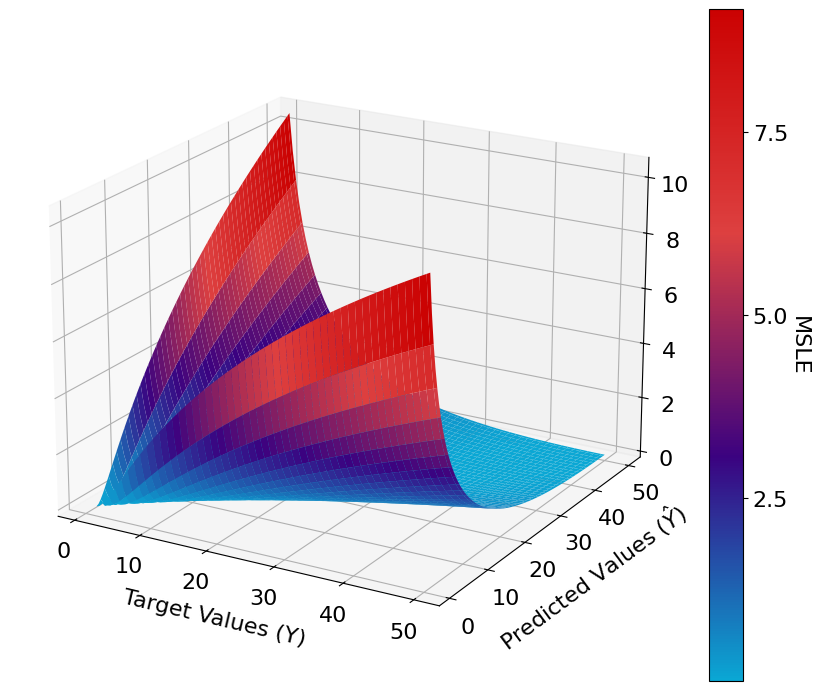
\includegraphics[width=0.6\textwidth]{figures/MSLE_3d_surface.png}
    
\end{figure*}

\begin{wrapfigure}{r}{0.5\textwidth}
    \centering
    \vspace{-10pt} 
    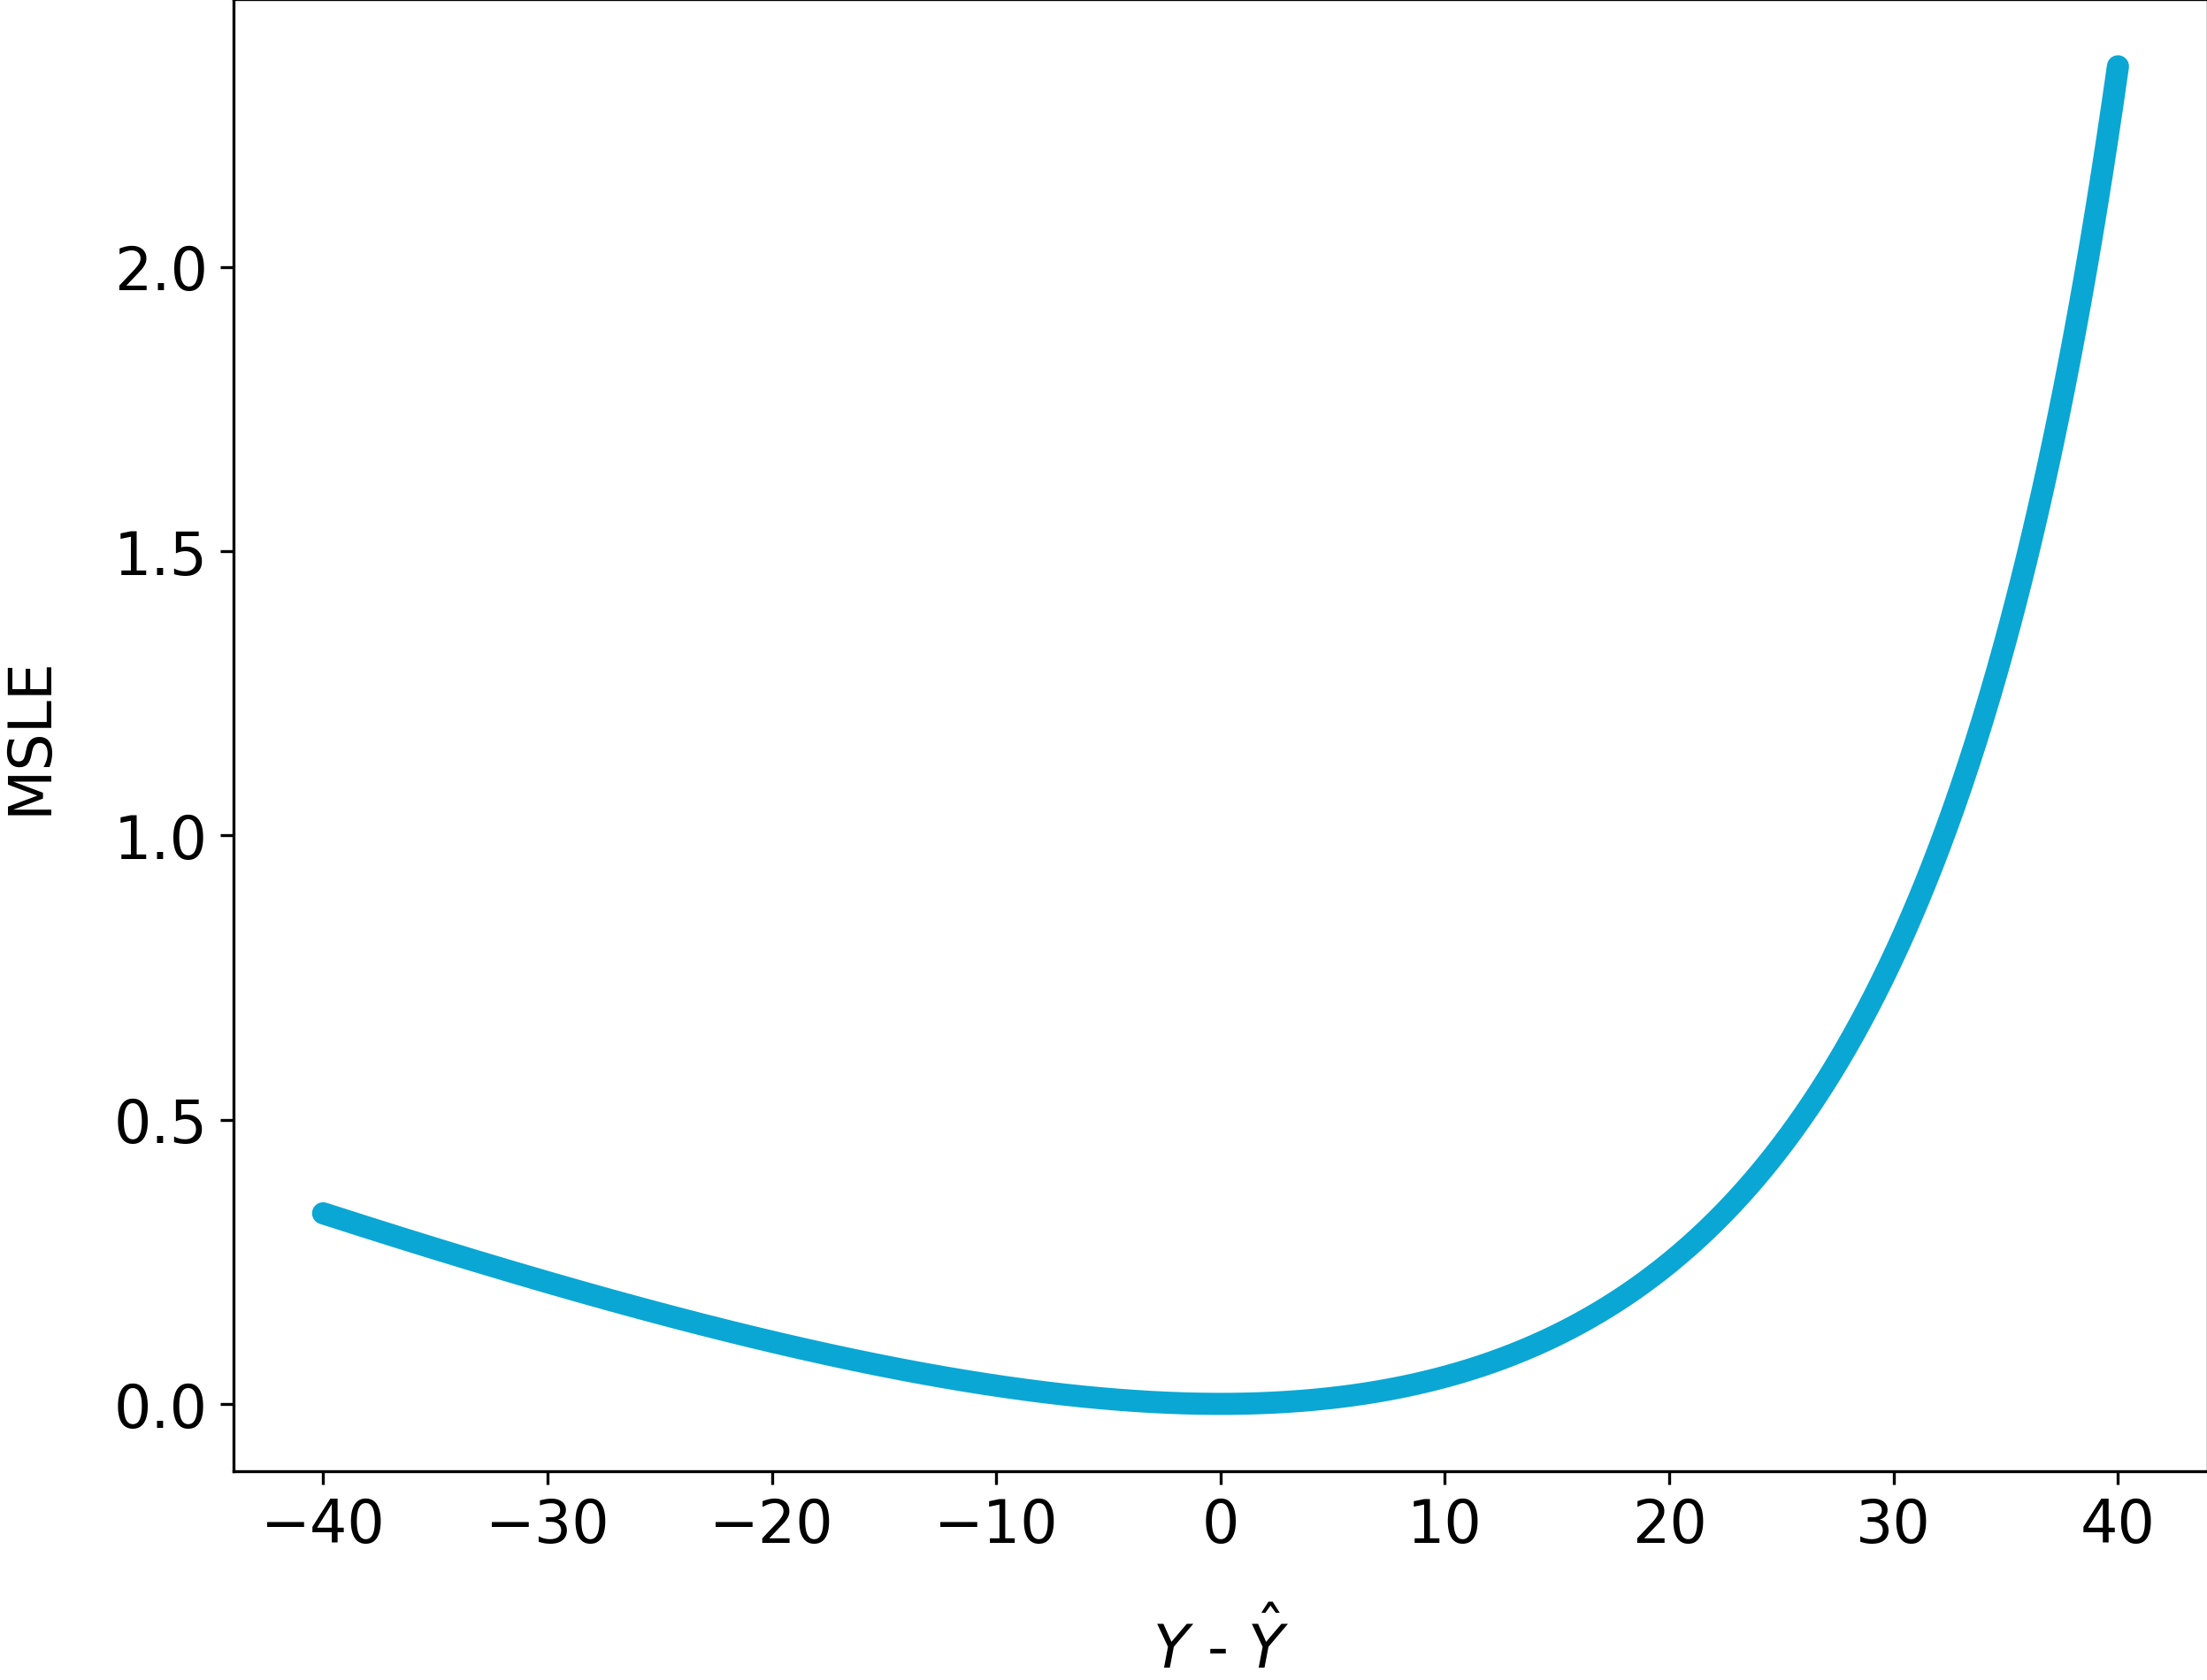
\includegraphics[width=0.45\textwidth]{figures/MSLE_cross_section.png} % Your figure goes here
    \vspace{-10pt} % Adjust vertical alignment if needed
\end{wrapfigure}

% Left text with the image on the right
\textbf{Figure 3.3 MSLE.} \underline{Top:} MSLE surface illustrates how the penalty varies across different target and predicted values, exhibiting a non-linear relationship.
\underline{Right:}  The cross-section reveals MSLE's asymmetric nature, penalizing underprediction more severely than overprediction. 



\orangebox{Did you know that...}
{MSLE uses logarithms to look at proportional differences instead of absolute ones. 
This makes it more sensitive to percentage errors. It also lowers the impact of large differences, unlike MSE, which treats them more strongly.}

\textbf{Other related metrics}

Related metrics for MSLE include Mean Absolute Log Error (MALE) and Root Mean Sqaured Log Error (RMSE). 

% ---------- RMSE ----------
\clearpage
\thispagestyle{regressionstyle}
\section{RMSE}
\subsection{Root Mean Squared Error}

Similarly to MSE, RMSE squares the difference between predictions and true values but takes the square root of the mean.
Simplifying its interpretation units since the error is returned in the natural units of the data.

% formula
\begin{center}
    \tikz{
        \node[inner sep=2pt, font=\Large] (a) {
            {
                $\displaystyle
                RMSE = \sqrt{\frac{1}{{\color{nmlred}n}} \sum_{t=1}^n \left({\color{nmlcyan}Y_t} - {\color{nmlpurple}\hat{Y}_t}\right)^2}
                $
            }
        };
        \draw[-latex,nmlred, semithick] ($(a.south)+(-0.2,0.3)$) to[bend left=20] node[pos=1, left] {number of samples} +(-1,-.7);
        \draw[-latex,nmlcyan, semithick] ($(a.south)+(1.5,0.6)$) to[bend right=15] node[pos=1, right] {actual value} +(1,-.5);
        \draw[-latex,nmlpurple, semithick] ($(a.north)+(2.5,-0.5)$) to[bend left=30] node[pos=1, right] {forecast value} +(1,.2); 
    }
\end{center}

The RMSE is always a positive value, with a smaller RMSE indicating better forecast accuracy.
Theoretically, RMSE belongs in the 0 to +infinity range. By squaring the differences, RMSE gives more weight to larger errors, making it sensitive to outliers.

\textbf{When to use RMSE?}

Use RMSE when you need a metric that penalizes larger errors more than smaller ones due to the squaring of the residuals and reports an
interpretable value in the same units as the target variable.

% strength and weakness box
\coloredboxes{
    \item Because RMSE is measured in the same units as the target variable, interpreting its magnitude is straightforward.
    \item The squaring of the errors ensures that larger errors have a greater impact on the RMSE value, which can be beneficial when large errors are particularly undesirable.
}
{
    \item Unlike some other metrics like R-squared and MAPE, RMSE does not provide a normalized measure, making it difficult to compare across different datasets without standardization.
}

\clearpage

\thispagestyle{customstyle}

\begin{figure*}[htbp]
    \centering
    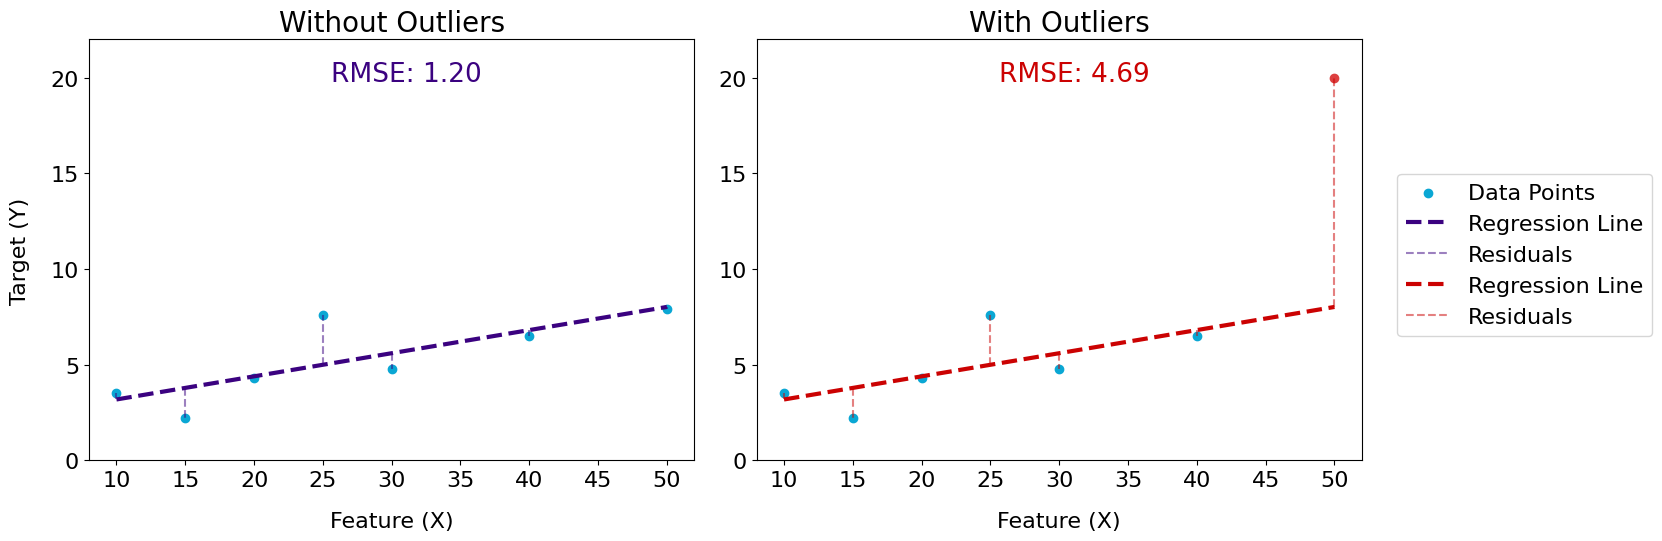
\includegraphics[width=0.95\textwidth]{figures/RMSE_sensitivity_outliers_plot.png} 
\end{figure*}

\begin{wrapfigure}{r}{0.45\textwidth}
    \centering
    \vspace{-5pt} 
    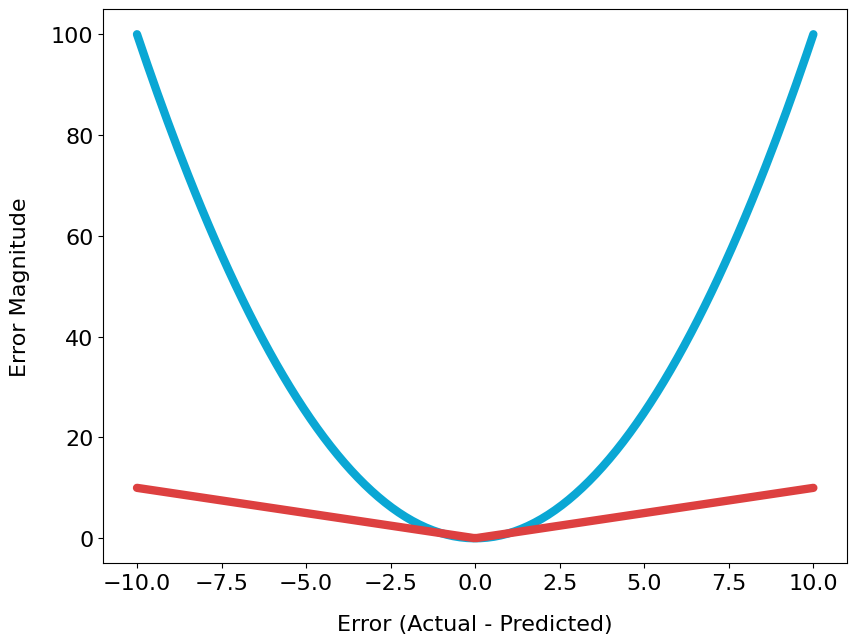
\includegraphics[width=0.40\textwidth]{figures/RMSE_comparison_2d_plot.png} 
    \vspace{-10pt} 
\end{wrapfigure}

\noindent
\textbf{Figure 3.4 RMSE.} \underline{Top:} RMSE is highly sensitive to outliers. The left plot shows RMSE without outliers, while the right plot demonstrates the increase in RMSE due to a single outlier. 
\underline{Right:} A visual comparison of MSE (blue) and RMSE (red). RMSE, due to its square root operation, often scales differently than MSE.

\vspace{10pt} 
\orangebox{Did you know that...}
{While there is no standard literature on normalizing RMSE, one approach is to divide the value by the range or mean. 
This normalized RMSE is commonly expressed as a percentage, known as the Coefficient of Variation (CV).}

\vspace{10pt} % Added spacing for better layout

\textbf{Other related metrics}
Metrics like Mean Absolute Error (MAE), Average Absolute Deviation (AAD), and Normalized Estimation Error Squared (NEES) are also used to evaluate model performance.

% ---------- RMSLE ----------
\clearpage
\thispagestyle{regressionstyle}
\section{RMSLE}
\subsection{Root Mean Squared Log Error}

RMSLE is a variation of the RMSE metric that is particularly useful when dealing with targets that have a wide range of values, such as those with an exponential growth pattern.
It measures the square root of the average of the squared logarithmic errors.

% formula
\begin{center}
    \tikz{
        \node[inner sep=2pt, font=\Large] (a) {
            {
                $\displaystyle
                RMSLE = \sqrt{\frac{1}{{\color{nmlred}n}} 
                        \sum_{t=1}^n
                        \left(
                            {log{({\color{nmlcyan}Y_t} + 1)}} -
                            {log{({\color{nmlpurple}\hat{Y}_t} + 1)}}
                        \right)^2}
                $
            }
        };
        \draw[-latex,nmlred, semithick] ($(a.south)+(-2.,0.3)$) to[bend right=15] node[pos=1, right] {number of samples} +(1,-.8);
        \draw[-latex,nmlcyan, semithick] ($(a.south)+(0.6,0.6)$) to[bend right=15] node[pos=1, right] {actual value} +(1,-.5);
        \draw[-latex,nmlpurple, semithick] ($(a.north)+(3.5,-0.5)$) to[bend left=20] node[pos=1, right] {forecast value} +(.4,.9); 
    }
\end{center}

RMSLE is always a positive value, with a smaller RMSLE indicating better forecast accuracy. Theoretically, RMSLE belongs in the 0 to +infinity range.
By using the logarithm, RMSLE dampens the effect of large outliers compared to RMSE.

\textbf{When to use RMSLE?}

RMSLE is best used when the target variables have a large range and an exponential growth pattern, such as population counts or sales figures over time.
It can be more appropriate than RMSE in these cases as it is less sensitive to large outliers.

% strength and weakness box
\coloredboxes{
    \item Handles large ranges of values well due to the logarithmic transformation.
    \item RMSLE penalizes underestimation more than overestimation, which can be beneficial in some use cases.
}
{
    \item RMSLE is not suitable for data with negative values or zero values, as the logarithm function is not defined for these.
    \item Interpretation can be less intuitive than RMSE, as the final value is in logarithmic scale.
}

\clearpage

\thispagestyle{customstyle}

\begin{figure*}[ht!]
    \centering
    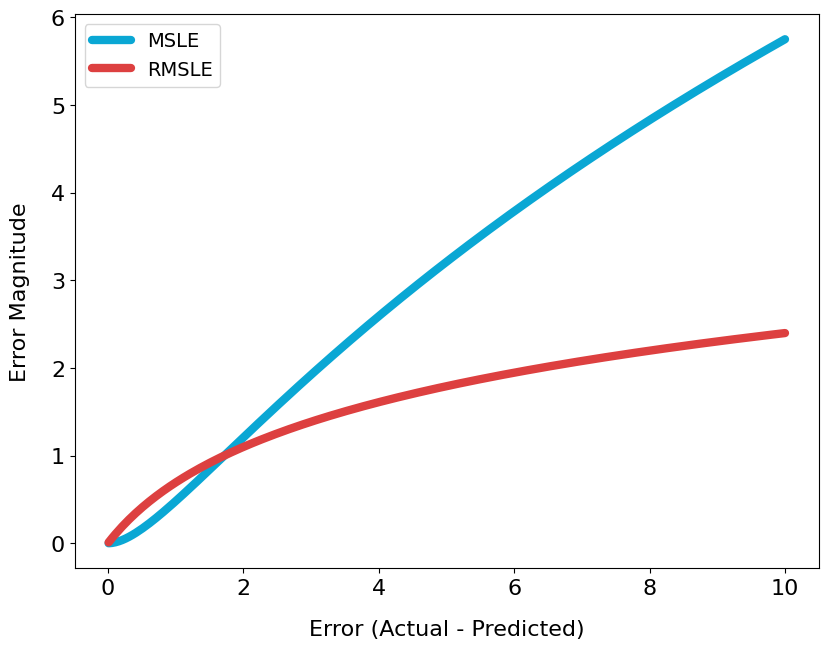
\includegraphics[width=0.6\textwidth]{figures/RMSLE_comparison_MSLE.png}
    % \caption{Caption}
\end{figure*}

% Left text with the image on the right
\textbf{Figure 3.5 RMSLE.} \underline{Top:} The MSLE curve grows quadratically, penalizing large relative errors more aggressively, 
while the RMSLE curve increases more slowly, smoothing out extreme values. Both metrics remain non-negative and centered around zero, 
with RMSLE being less sensitive to large errors. 

\orangebox{Did you know that...}
{RMSLE gained popularity during the 2019 ASHRAE - Great Energy Predictor III competition on Kaggle. 
An earlier appearance can be noted in the 2017 Mercari Price Suggestion Challenge on Kaggle as well.}

\textbf{Other related metrics}
RMSLE is suited to data that has exponential growth and in usecases like demand forecasting, metrics that are similar in 
fashion are Mean Squared Logarithmic Error (MSLE), Mean Absolute Percentage Error (MAPE) , Huber Loss and Quantile Loss. 
% ---------- MAPE ----------
\clearpage
\thispagestyle{regressionstyle}
\section{MAPE}
\subsection{Mean Absolute Percentage Error}

MAPE is one of the most widely used measures of forecast accuracy due to its scale independence and interoperability.
It is derived from the Mean Absolute Error (MAE), adjusted to provide a percentage measure, making it easier to interpret and compare across different datasets and contexts.

% formula
\begin{center}
    \tikz{
        \node[inner sep=2pt, font=\Large] (a) {
            {
                $\displaystyle
                MAPE = \frac{1}{{\color{nmlred}n}} \sum_{t=1}^n \left| \frac{Y_t - \color{nmlpurple}\hat{Y}_t}{\color{nmlcyan}Y_t} \right| \times 100
                $
            }
        };
        \draw[-latex,nmlred, semithick] ($(a.south)+(-0.9,0.2)$) to[bend left=15] node[pos=1, left] {number of samples} +(-1,-.5);
        \draw[-latex,nmlpurple, semithick] ($(a.north)+(1.7,0.0)$) to[bend left=15] node[pos=1, right] {forecast value} +(1,.5); 
        \draw[-latex,nmlcyan, semithick] ($(a.south)+(1.2,0.2)$) to[bend right=15] node[pos=1, right] {actual value} +(1,-.5);
    }
\end{center}

When the forecasted values $\hat{Y_{t}}$ are equal to the actual values $Y_{t}$ for all data points, MAPE is 0\% indicating a perfect forecast with no error.
However, when the relationship between the actual values and predicted values are very different, the percentage error becomes extremely large.

\textbf{When to use MAPE?}

MAPE is useful when the value of the error on it's own is not as important as its relative magnitude compared to the actual target values.
It is not feasible when actual values can be 0. Additionally, MAPE is beneficial when it serves as a meaningful business metric.

% strength and weakness box
\coloredboxes{
    \item Scale-independent and easy interpretation as a percentage error.
}
{
    \item Undefined when $Y_{t} = 0$
    \item MAPE penalizes negative errors $(\hat{Y_{t}} > Y_{t})$ more than positive errors. This makes it biased since, optimizing for MAPE systematically selects the method with lower forecasts.
}

\clearpage

\thispagestyle{customstyle}

\begin{figure*}[ht!]
    \centering
    \includegraphics[width=0.6\textwidth]{figures/MAPE_3d_surface.png}
    % \caption{Caption}
\end{figure*}


\begin{wrapfigure}{r}{0.5\textwidth}
    \centering
    \vspace{-10pt} % Adjust vertical alignment if needed
    \includegraphics[width=0.45\textwidth]{figures/MAPE_cross_section.png} % Your figure goes here
    \vspace{-10pt} % Adjust vertical alignment if needed
\end{wrapfigure}


% Left text with the image on the right
\textbf{Figure 3.6 MAPE.} Illustrates the drawbacks of MAPE. It produces extremely large values (red area) when the relationship between
targets and predicted values is significantly different. \underline{Top:} The rate of change of MAPE is non-linear.
\underline{Right:} Clearly shows MAPE's asymmetry in relation to over- and under-predicting the target variable when optimizing for MAPE.

\orangebox{Did you know that...}
{MAPE is not translation invariant. This means that if we add a constant to all actual and prediction values, the error will be different.
In math terms, it means that $MAPE(Y_{t} + c, \hat{Y_{t}} + c) \not= MAPE(Y_{t}, \hat{Y_{t}})$ , where $c$ is a constant.}


\textbf{Other related metrics}
To overcome these issues with MAPE, there are some other measures proposed in the literature: Mean Absolute Scaled Error (MASE),
Symmetric Mean Absolute Percentage Error (sMAPE), Mean Directional Accuracy (MDA), Mean Arctangent Absolute Percentage Error (MAAPE).

% ---------- sMAPE ----------
\clearpage
\thispagestyle{regressionstyle}
\section{sMAPE}
\subsection{Symmetric Mean Absolute Percentage Error}

sMAPE is a variant of the popular metric MAPE and addresses some of its shortcomings. Unlike MAPE, sMAPE has both a lower and an upper bound and is also better
at handling data with target values that can be zero.

% formula
\begin{center}
	\tikz{
		\node[inner sep=2pt, font=\Large] (a) {
			{
				$\displaystyle
				sMAPE = \frac{1}{{\color{nmlred}n}} \sum_{t=1}^n \frac{\left| {\color{nmlcyan}Y_t} - {\color{nmlpurple}\hat{Y}_t} \right|}{({|\color{nmlcyan}Y_t}| + {|\color{nmlpurple}\hat{Y}_t}|)/2} \times 100
				$
			}
		};
		\draw[-latex,nmlred, semithick] ($(a.south)+(-0.8,0.3)$) to[bend left=15] node[pos=1, left] {number of samples} +(-1,-.5);
		\draw[-latex,nmlcyan, semithick] ($(a.north)+(0.6,0.0)$) to[bend right=15] node[pos=1, left] {actual value} +(-1,.5);
		\draw[-latex,nmlpurple, semithick] ($(a.north)+(1.8,0.0)$) to[bend left=15] node[pos=1, right] {forecast value} +(1,.5); 
	}
\end{center}

sMAPE ranges from 0\% to 200\%, with 0\% indicating a perfect forecast and 200\% indicating the worst possible forecast. There is another sMAPE version without the factor of 0.5 in the denominator, which makes the metric range between 0\% and 100\%.

\textbf{When to use sMAPE?}

sMAPE is a good choice when you want some of the benefits of MAPE, like percentage interpretation, but don't want its shortcomings like producing extremely large values when the relationship between
targets and predicted values are very different.

% strength and weakness box
\coloredboxes{
    \item Can handle target values equal to zero.
    \item Has both a lower and an upper bound.
}
{
    \item Undefined when $|Y_{t}| = |\hat{Y_{t}}| = 0$
    \item sMAPE is not symmetric to over- and under-forecasts. For example, if $Y_{t} = 100$ and in one case we have $\hat{Y_{t}} = 90$, this gives ansMAPE of 4.76\%; whereas if $\hat{Y_{t}} = 110$, then the sMAPE would be 5.26\%.
}

\clearpage

\thispagestyle{customstyle}

\begin{figure*}[ht!]
    \centering
    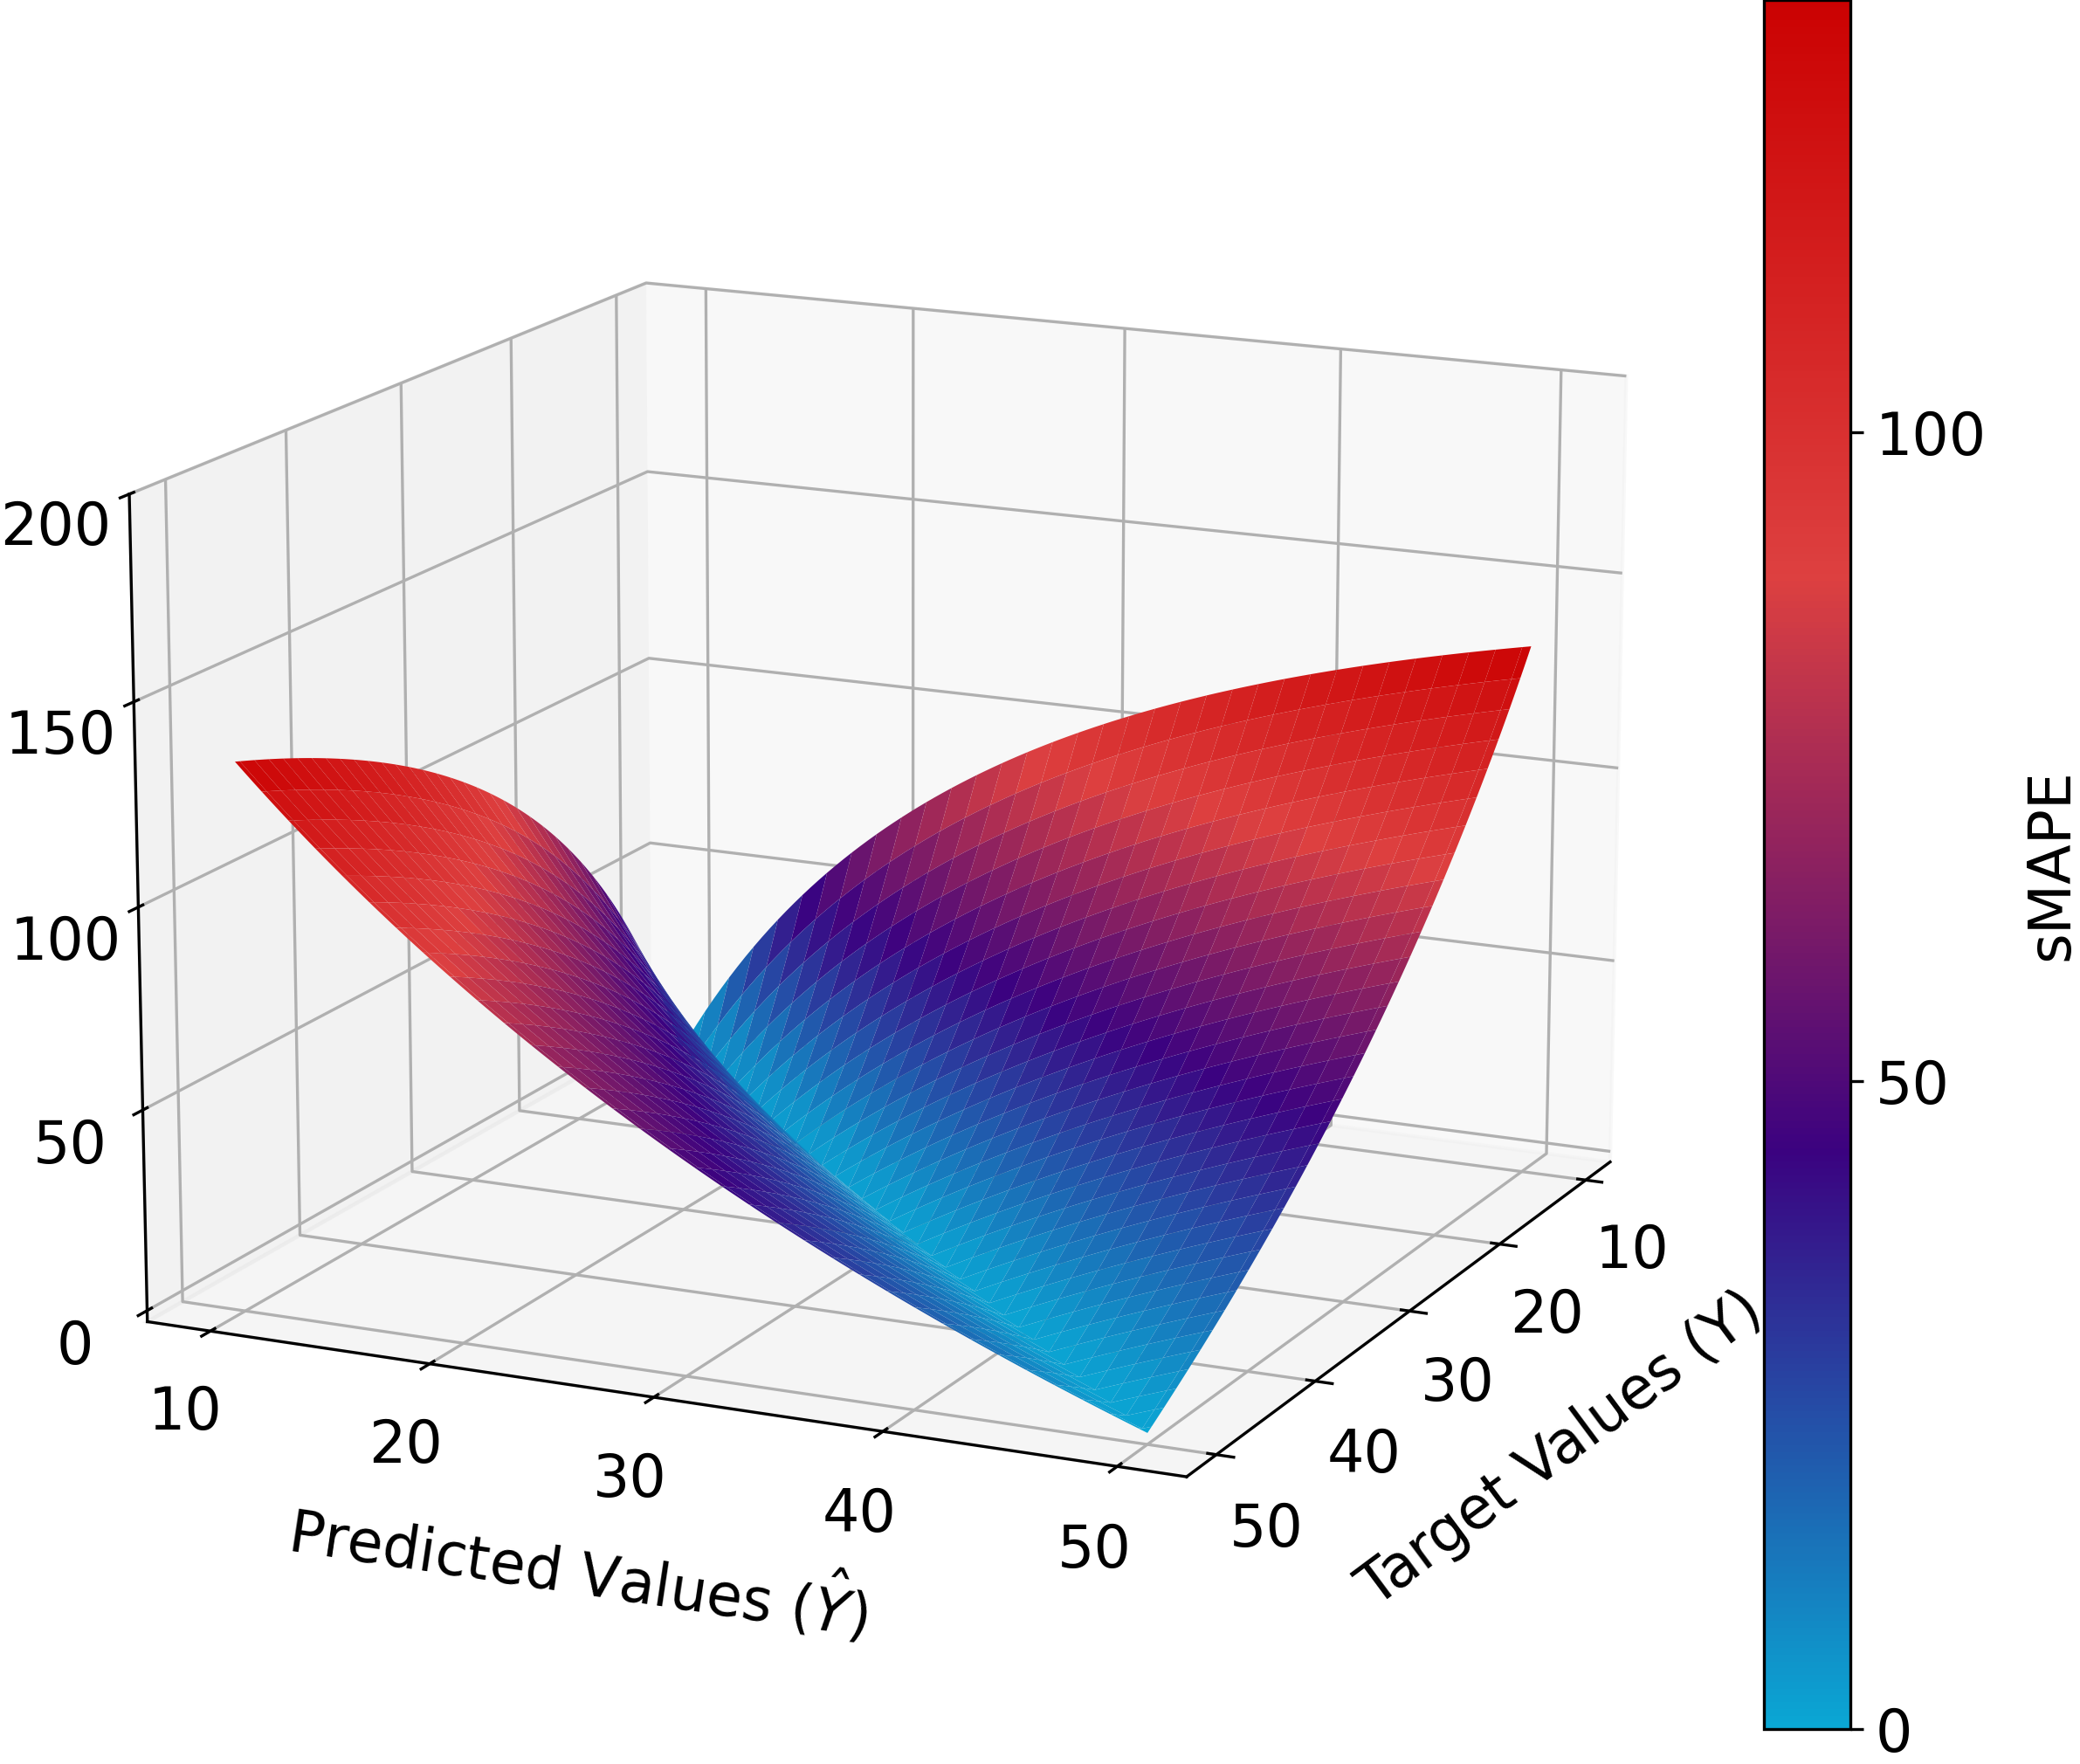
\includegraphics[width=0.6\textwidth]{figures/sMAPE_3d_surface.png}
    % \caption{Caption}
\end{figure*}

\begin{wrapfigure}{r}{0.5\textwidth}
    \centering
    \vspace{-10pt} % Adjust vertical alignment if needed
    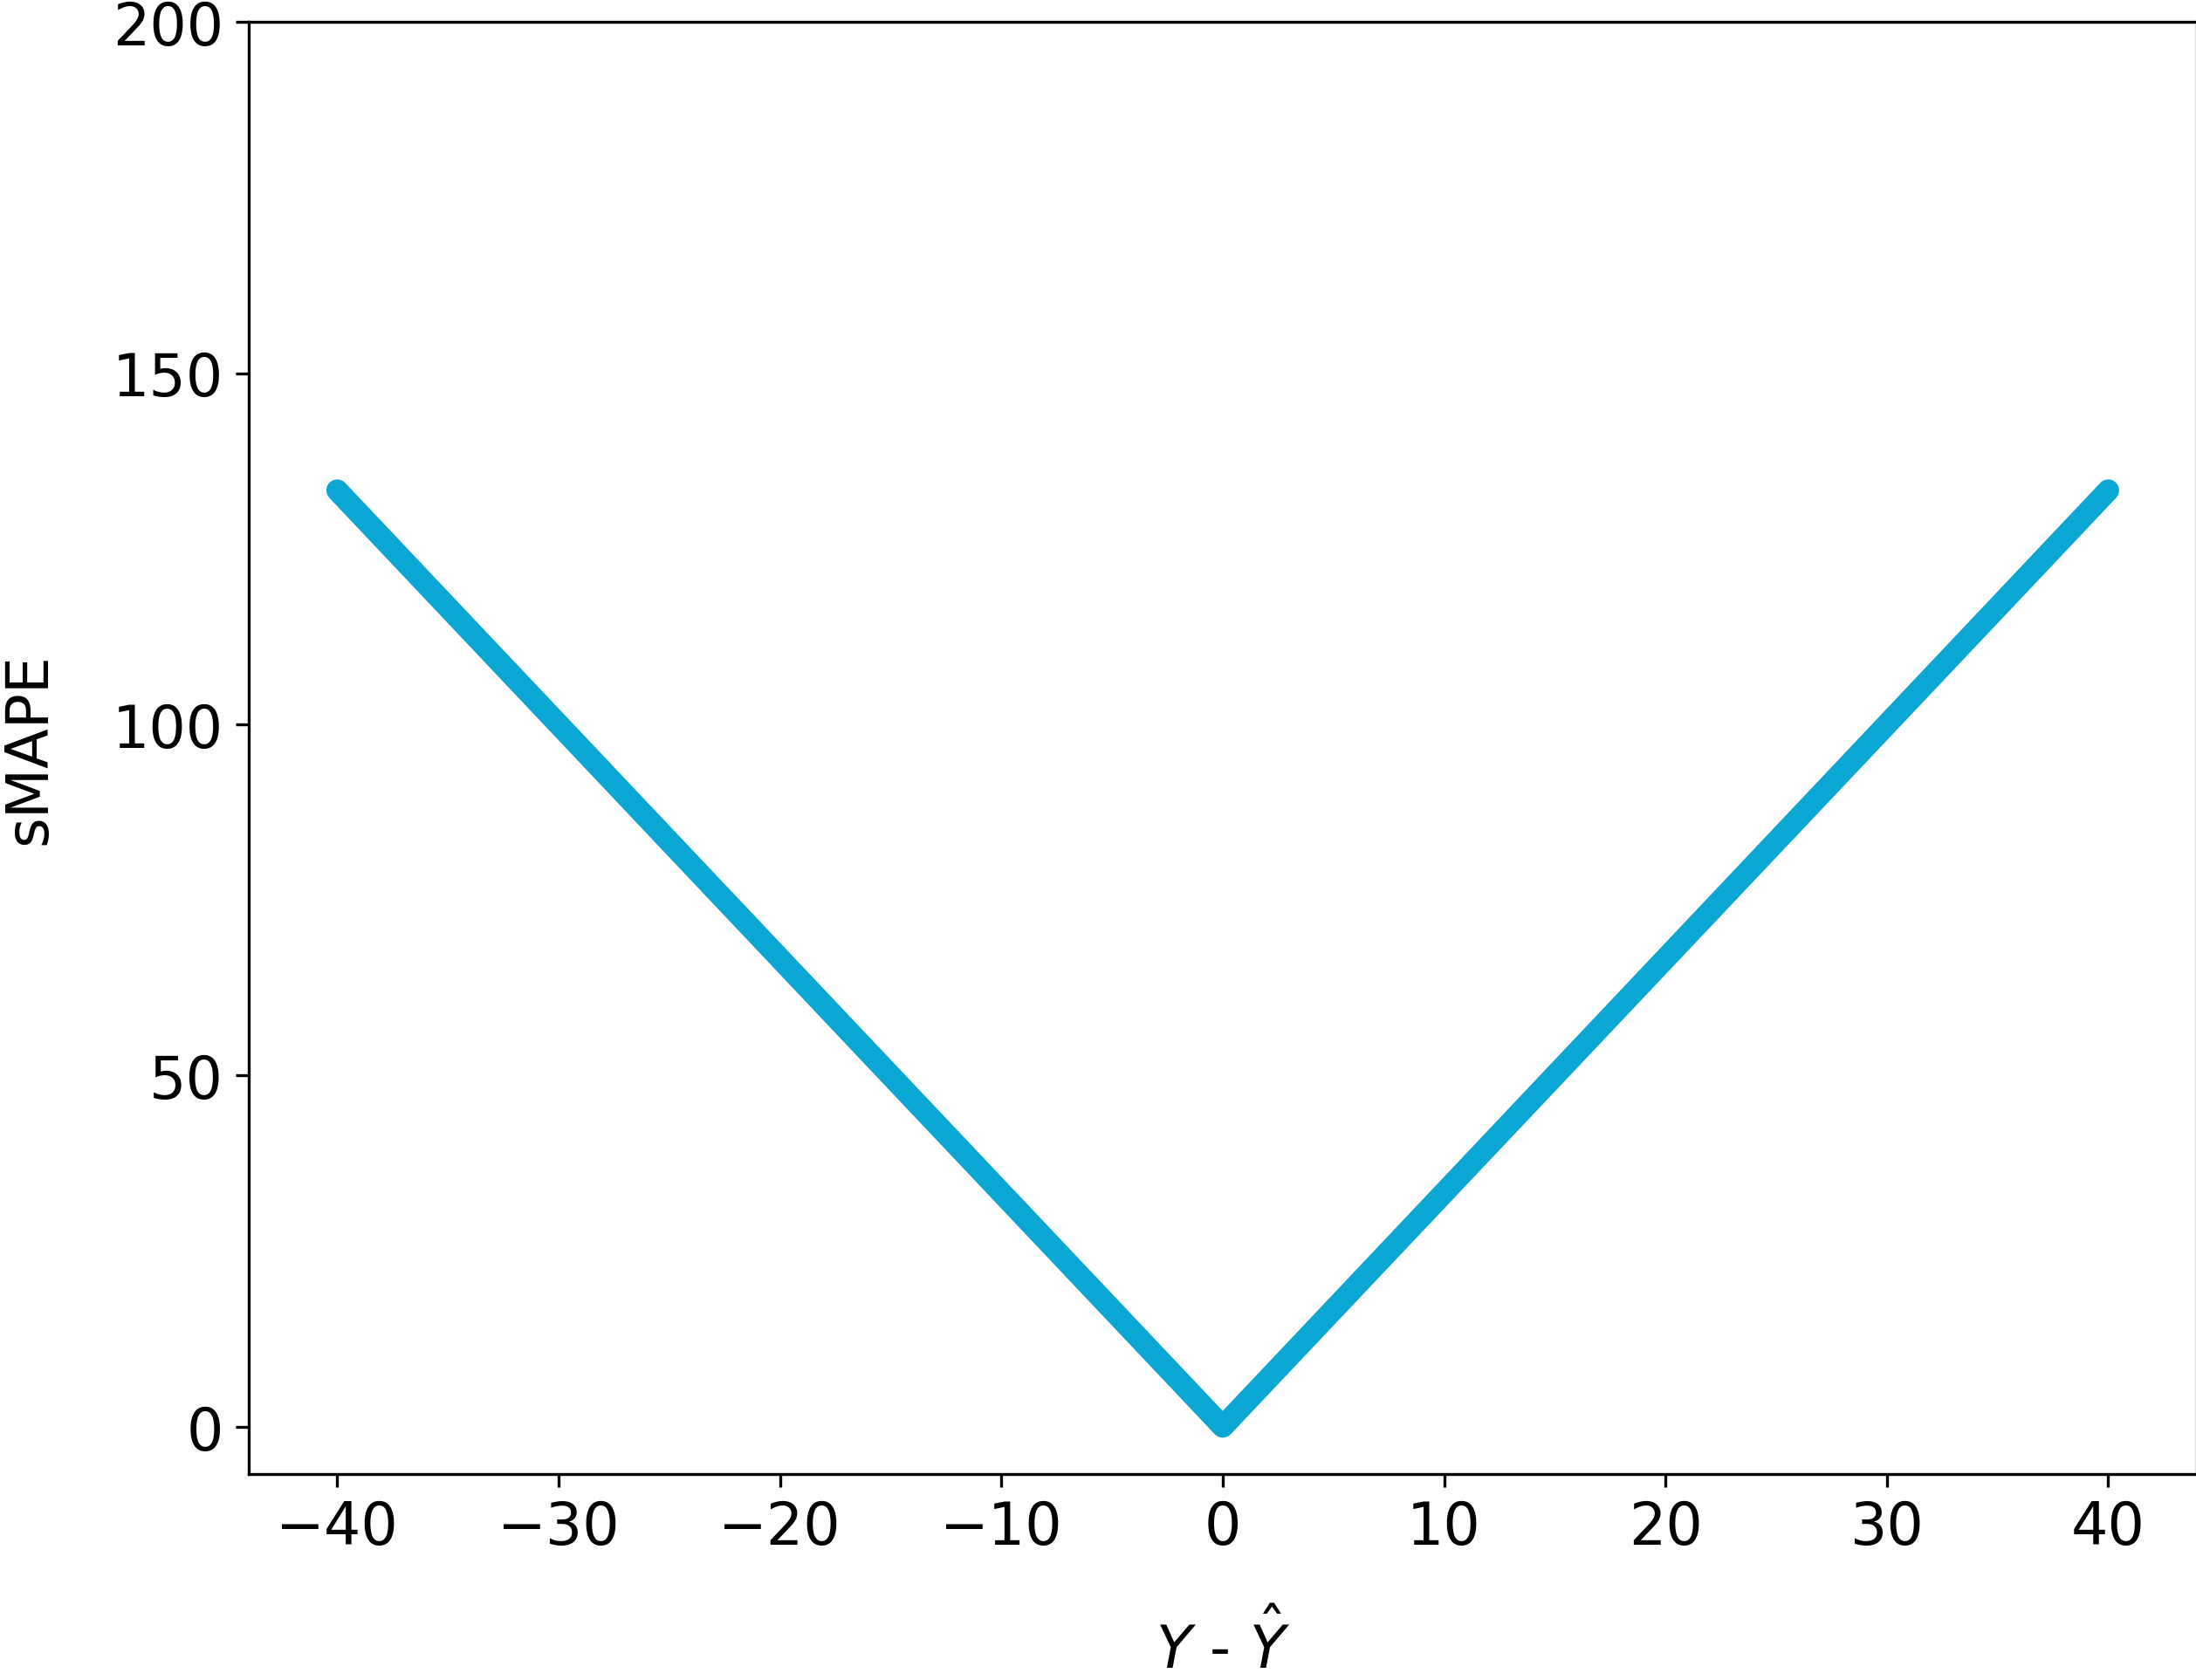
\includegraphics[width=0.45\textwidth]{figures/sMAPE_cross_section.png} % Your figure goes here
    \vspace{-10pt} % Adjust vertical alignment if needed
\end{wrapfigure}

\sloppy
\textbf{Figure 3.7 sMAPE.}Unlike MAPE, sMAPE remains bounded but still exhibits extreme values 
(red area) when the difference between targets and predictions is large. \underline{Top:} Shows the non-linear response of sMAPE to deviations from the true value.
\underline{Right:} Demonstrates sMAPE’s symmetric nature, where over- and under-predictions result in the same error magnitude.
% Source : https://scholarworks.utep.edu/cgi/viewcontent.cgi?article=1865&context=cs_techrep
\sloppy
\orangebox{Did you know that...}
{SMAPE explains why the geometric mean often produces the best forecast combination. 
When you have two forecasts, \( x \) and \( y \), you need to find a single estimate, \( z \), that minimizes the total SMAPE error:
\[
s(x,z)+s(y,z) = \frac{|x - z|}{x + z} + \frac{|y - z|}{y + z}
\]
The best choice for \( z \) is the geometric mean:
\[
z = \sqrt{x \cdot y}
\]
This result matters in real-world forecasting. Many competitions and industry applications use this approach to improve forecasting accuracy.}

% ---------- wMAPE ----------
\clearpage
\thispagestyle{regressionstyle}
\section{wMAPE}
\subsection{Weighted Mean Absolute Percentage Error}

wMAPE is an extension of the MAPE metric, where MAPE is treated as a weighted arimetric mean. The original formula shows weights $w_{t}$ but most of the time this weights are replaced
with actual values $Y_{t}$.

% formula
\begin{center}
    \tikz{
        \node[inner sep=2pt, font=\Large] (a) {
            {
                $\displaystyle
                wMAPE = \frac{\sum_{t=1}^n |{\color{nmlcyan}Y_t} - {\color{nmlpurple}\hat{Y}_t}|}{\sum_{t=1}^n |{\color{nmlcyan}Y_t}|} \times 100
                $
            }
        };
        \draw[-latex,nmlcyan,semithick] ($(a.north)+(0.8,-0.1)$) to[bend right=15] node[pos=1, left] {actual value} +(-1,.5);
        \draw[-latex,nmlpurple, semithick] ($(a.north)+(2.0,0.0)$) to[bend left=15] node[pos=1, right] {forecast value} +(1,.5); 
    }
\end{center}


wMAPE ranges from 0\% to +infinity, with 0\% indicating a perfect forecast. Unlike MAPE and even sMAPE, wMAPE doesn't have an issue when the denominator being zero,
only if $\sum_{t=1}^{N}|Y_{t}| = 0$ which is unlike since that would mean every $Y_{t}$ is zero. We can think about wMAPE as a version of MAE that is normalized by the sum of
actuals rather than number of observations.

\textbf{When to use wMAPE?}

wMAPE is a good choice when you want some of the characteristics of MAPE, like percentage interpretation and unbound upper limit but don't want it's 'infinity error' issue.

% strength and weakness box
\coloredboxes{
    \item Robustness to zero and near-zero actuals.
    \item Scale-independent metric.
}
{
    \item Not a true percentage error
}

\clearpage 
\thispagestyle{customstyle}
%inspiration for this : https://www.baeldung.com/cs/mape-vs-wape-vs-wmape
To illustrate the real-world use of WMAPE compared to MAPE, let's look at a business scenario. 
Table 3.8 shows the sales growth for each channel, the forecast errors made by the predicting machine learning model,
and the weight of each channel based on the revenue it generates. 

{
\small
\noindent
\begin{tabular}{l r r c c c }
\hline
\textbf{Channel} & \textbf{Actual} & \textbf{Forecast} & \textbf{MAPE (\%)} & \textbf{Revenue Wt(\%)} & \textbf{wMAPE (\%)} \\
\hline
B2B          & 1,10,000    & 99,010     & 9.1   & 8.3   & 0.76 \\
Online       & 90,000      & 79,990     & 11.1  & 6.8   & 0.75 \\
Marketplace  & 1,20,000    & 1,10,040   & 8.3   & 9.1   & 0.76 \\
Retail       & 10,00,000   & 9,00,000   & 10.0  & 75.8  & 7.58 \\
\hline
\end{tabular}
}
\setcounter{figure}{7}
\begin{figure*}[ht!]
    \centering
    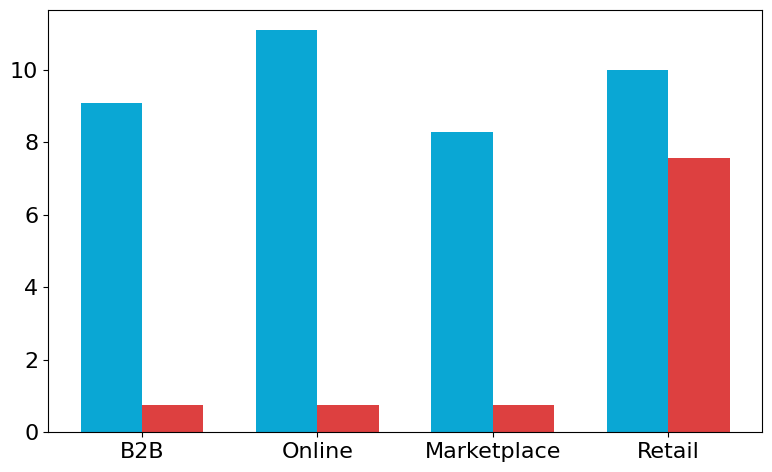
\includegraphics[width=1.0\textwidth]{figures/wMAPE_compare_MAPE.png}
    \caption{Channel-wise Sales Forecast Errors: WMAPE (red)}
\end{figure*}

At first glance, if you only look at the MAPE (blue), it might seem like the model struggles equally with each channel, 
showing an error margin of about 10 percent. 

However, when you consider WMAPE (red), you can clearly see the risk these errors pose for each channel. 

The retail channel accounts for 75 percent of the revenue, so even the smallest error can have a significant impact on business strategy. While MAPE shows all the errors, 
WMAPE helps highlight which errors should be addressed first. This is illustrated in Fig. 3.8.




% ---------- MASE ----------
\clearpage
\thispagestyle{regressionstyle}
\section{MASE}
\subsection{Mean Absolute Scaled Error}

MASE is a scale-independent metric that compares the absolute errors of a forecast model to the absolute errors of a naive forecast.
This makes MASE particularly useful for comparing the performance of models across different datasets or when the scale of the target variable changes.
\vspace{-1em}
% formula
\begin{center}
    \tikz{
        \node[inner sep=2pt, font=\Large] (a) {
            {
                $\displaystyle
                MASE = \frac{1}{{\color{nmlred}n}} \sum_{t=1}^n \frac{|{\color{nmlcyan}Y_t} - {\color{nmlpurple}\hat{Y}_t}|}{\frac{1}{n-1} \sum_{t=2}^n |{\color{nmlcyan}Y_t} - {\color{nmlcyan}Y_{t-1}}|}
                $
            }
        };
        \draw[-latex,nmlred, semithick] ($(a.south)+(-1.5,0.2)$) to[bend left=15] node[pos=1, left] {number of samples} +(-1,-.5);
        \draw[-latex,nmlpurple, semithick] ($(a.north)+(2.4,-0.05)$) to[bend left=15] node[pos=1, right] {forecast value} +(1,.5); 
        \draw[-latex,nmlcyan,semithick] ($(a.north)+(1.2,-0.1)$) to[bend right=15] node[pos=1, left] {actual value} +(-1,.5);
    }
\end{center}
\vspace{-1em}
MASE values less than 1 indicate that the forecast model outperforms the naive forecast, while values greater than 1 indicate the opposite.
MASE is unbounded on the positive side, with 0 representing a perfect forecast.

\textbf{When to use MASE?}

MASE is great for evaluating forecast performance against a baseline model. Because of its scale-independent characteristic, it is also suitable for comparing the accuracy
of forecasts across datasets with different units or magnitudes.

% strength and weakness box
\coloredboxes{
    \item Scale-independent, allowing for fair comparisons across datasets.
    \item Provides a clear benchmark for model performance relative to a naive forecast.
    \item Unlike percentage-based metrics such as MAPE, MASE avoids division by zero issues.
    \item MASE penalizes positive and negative forecast errors equally, and it treats errors in large and small forecasts with equal weight.

}
{
    \item Requires defining a suitable naive forecast method.    
    \item MASE may not be as intuitive to interpret as some other metrics like MAE or MAPE.
}

% \clearpage
\orangebox{Did you know that...}
{MASE was created by Anne B. Koehler and Rob J. Hyndman, co-author of the book Forecasting: Principles and Practice, widely regarded as one of the definitive resources in forecasting.}

% ---------- MDA ----------
\clearpage
\thispagestyle{regressionstyle}
\section{MDA}
\subsection{Mean Directional Accuracy}

MDA is a metric used to evaluate the performance of forecasting models in terms of their ability to correctly predict the direction of change in the target variable,
rather than the magnitude of the change.

% formula
\begin{center}
    \tikz{
    \node[inner sep=2pt, font=\Large] (a) {
        {
            $\displaystyle
            MDA = \frac{1}{{\color{nmlred}n}} \sum_{t=1}^{n} {\color{nmlgreen}\mathds{1}}_{{\color{nmlyellow}sign}({\color{nmlcyan}y_t} - {\color{nmlcyan}y_{t-1}}) == {\color{nmlyellow}sign}({\color{nmlpurple}\hat{y}_t} - {\color{nmlcyan}y_{t-1}})}
            $
        }
    };

    % Draw arrows for annotations
    \draw[-latex, nmlred, semithick] ($(a.south)+(-2.4,0.4)$) to[bend right=5] node[pos=1, left] {number of samples} +(-1,-.85);
    \draw[-latex,nmlcyan,semithick] ($(a.north)+(0.2,-0.6)$) to[bend right=15] node[pos=1, left] {actual value at time t} +(-1,1);
    \draw[-latex, nmlpurple, semithick] ($(a.north)+(3,-0.6)$) -- +(0,0.65) node[above, yshift=2pt] {forecast value at time $t$};
    \draw[-latex, nmlgreen, semithick] ($(a.south)+(-0.8,0.6)$) -- +(0,-0.7) node[below, yshift=-2pt] {indicator function};
    \draw[-latex, nmlyellow, semithick] ($(a.south)+(2.6,0.5)$) -- +(0,-0.6) node[below, yshift=-2pt] {$sign(\cdot)$ function};
    }
\end{center}

To compute it we count the number of times the predicted value has the same sign as the actual value divided by the total number of samples. MDA ranges from 0 to 1, with 1 indicating
that the model correctly predicted the direction of change for all data points, and 0 indicating that the model
always predicted the opposite direction.

\textbf{When to use MDA?}

MDA is useful when the ability to predict the direction of change is more important than the precise magnitude of the forecast. This can be the case in finance and economics,
where correctly identifying the directional movement of variable can be more valuable than accurately predicting the exact price movement.

% strength and weakness box
\coloredboxes{
    \item Provides a simple, interpretable metric that is not affected by the scale of the target variable.

}
{
    \item MDA does not provide any information about the magnitude of the errors, only the direction.
}

% ---------- MPD ----------
\clearpage
\thispagestyle{regressionstyle}
\section{MPD}
\subsection{Mean Poisson Deviance}

MPD is a metric used to evaluate the performance of regression models when the target variable follows a Poisson distribution. This distribution is common for count data, such as the number
of events occurring in a fixed time or space (e.g., website clicks per hour, phone calls received per day).

% formula
\begin{center}
    \tikz{
        \node[inner sep=2pt, font=\Large] (a) {
            {
                $\displaystyle
                MPD = \frac{1}{{\color{nmlred}n}} \sum_{t=1}^{n} 2 \left( {\color{nmlpurple}Y_i} log ( \frac {\color{nmlpurple}Y_i}{\color{nmlcyan}\hat{Y}_i} ) - ( {\color{nmlpurple}Y_i} - {\color{nmlcyan}\hat{Y}_i} ) \right)
                $
            }
        };
        \draw[-latex,nmlred, semithick] ($(a.south)+(-2.2,0.2)$) to[bend left=15] node[pos=1, left] {number of samples} +(-1,-0.5);
        \draw[-latex,nmlpurple, semithick] ($(a.north)+(1.3,0.0)$) to[bend left=15] node[pos=1, right] {actual value} +(1,.5); 
        \draw[-latex,nmlcyan, semithick] ($(a.south)+(1.3,0)$) to[bend right=15] node[pos=1, right] {predicted value} +(1,-0.5);
    }
\end{center}

MPD ranges from 0 to +infinity, with 0 indicating a perfect model fit for count data. It is particularly sensitive to the underlying Poisson distribution characteristics.

\textbf{When to use MPD?}

When the target variable represents counts, and when the predictions are constrained to be non-negative.

% strength and weakness box
\coloredboxes{
    \item Directly relates to the Poisson distribution, making it interpretable when dealing with count data.
    \item Accounts for relative errors. Larger deviations matter more, e.g., \( MPD(y=100, \hat{y}=150) > MPD(y=1.0, \hat{y}=1.5) \).
}
{
    \item Sensitive to Zero Counts.
    \item Requires positive targets and predictions.
}

% ---------- MGD ----------
\clearpage
\thispagestyle{regressionstyle}
\section{MGD}
\subsection{Mean Gamma Deviance}

MGD is a metric for evaluating regression models when the target variable follows a Gamma distribution. This distribution is often used for modeling continuous positive data with a
positive right-skewed distribution, such as insurance claims, response times, or medical expenditures.

% formula
\begin{center}
    \tikz{
    \node[inner sep=2pt, font=\Large] (a) {
        {
            $\displaystyle
            MGD = \frac{1}{{\color{nmlred}n}} \sum_{i=0}^{{n-1}} 2 \left( {\color{nmlcyan}y_i} log\left(\frac{\color{nmlcyan}y_i}{\color{nmlpurple}\hat{y}_i}\right) - ({\color{nmlcyan}y_i} - {\color{nmlpurple}\hat{y}_i}) \right)
            $
        }
    };
    
    \draw[-latex,nmlred, semithick] ($(a.south)+(-2.5,0.2)$) to[bend left=15] node[pos=1, left] {number of samples} +(-1,-.5);
    \draw[-latex, nmlcyan, semithick] ($(a.north)+(1.2,-0.2)$) to[bend left=15] node[pos=1, right] {actual value} +(1,.5);
    \draw[-latex, nmlpurple, semithick] ($(a.south)+(1.2,0.2)$) to[bend right=15] node[pos=1, right] {predicted value} +(1,-.5);
}
\end{center}

MGD ranges from 0 to +infinity, with 0 indicating a perfect model fit for count data.

\textbf{When to use MGD?}

When the target variable is strictly positive and has a right-skewed distribution (e.g., durations, financial costs).

% strength and weakness box
\coloredboxes{
    \item MGD is tailored for right-skewed data. It gandles continuous positive data with increasing variance efficiently.
    \item MGD penalizes predictions proportionally to the magnitude of the target variable, e.g., \( MGD(y=100, \hat{y}=150) = MGD(y=1.0, \hat{y}=1.5) \).
}
{
    \item Targets as well as predictions must be strictly positive, limiting the metric’s compatibility with some models.
    \item Not appropriate for data that doesn't follow a Gamma-like structure
}

% ---------- R-squared ----------
\clearpage
\section{R-squared}
\subsection{R-squared}
\thispagestyle{regressionstyle}

R-squared needs little introduction; it's featured in every statistics book. Also known as the coefficient of determination, it's commonly introduced as a measure that quantifies the amount of variability explained by the regression model.

\begin{center}
    \tikz{
        \node[inner sep=2pt, font=\Large] (a) {
            {
                $\displaystyle
                R^2 = 1 - \frac{\sum_{t=1}^n (Y_t - {\color{nmlpurple}\hat{Y}_t})^2}{\sum_{t=1}^n ({\color{nmlcyan}Y_t} - {\color{teal!70!green}\bar{Y}})^2}
                $
            }
        };
        
        \draw[-latex,nmlpurple, semithick] ($(a.north)+(2.1,0)$) to[bend left=15] node[pos=1, right] {Predicted value} +(1,.5); 
        \draw[-latex,teal!70!green, semithick] ($(a.south)+(2.1,0.1)$) to[bend right=15] node[pos=1, right] {Mean of targets} +(1,-.5); 
        \draw[-latex,nmlcyan, semithick] ($(a.south)+(1,0.1)$) to[bend left=15] node[pos=1, left] {Target value} +(-1,-.5); 
    }
\end{center}

However, it may be easier to think of R-squared as a way to scale MSE between a perfect model and one that always predicts the mean. A score of 1.0 means $Y_t$ and $\hat{Y}_t$ are equal. Despite its name, R-squared can be negative if the model performs worse than just predicting the mean.

\textbf{When to use R-squared?}

R-squared can be more intuitive than MAE, MSE, RMSE, and other scale-dependent metrics since it can be expressed as a percentage, whereas the latter have arbitrary ranges.

\coloredboxes{
    \item Easy Interpretation. Especially when interpreted as a scaled MSE.
    \item R-squared is widely accepted in statistical analysis and research, making it a standard choice for evaluating model performance.
}
{
    \item Just like MSE, R-squared can be sensitive to outliers, as large errors have a greater impact.
    \item Be cautious about which value of $\bar{Y}$ to use. Most implementations default to $\bar{Y}_{\text {test }}$ which can lead to information leakage. It is advisable to use $\bar{Y}_{\text {train }}$ instead.
}


\clearpage
\thispagestyle{customstyle}

\begin{wrapfigure}{r}{0.45\textwidth}
    \centering
    \vspace{-5pt} 
    \includegraphics[width=0.40\textwidth]{figures/R2_explained.png} 
    \vspace{-10pt} 
\end{wrapfigure}


\begin{wrapfigure}{r}{0.5\textwidth}
    \centering
    \vspace{-10pt} % Adjust vertical alignment if needed
    \includegraphics[width=0.45\textwidth]{figures/R2_3d_surface.png} % Your figure goes here
    \vspace{-10pt} % Adjust vertical alignment if needed
\end{wrapfigure}

% Left text with the image on the right
\textbf{Figure 2.15 R-Squared.} \underline{Top:} The
areas of the purple squares
represent the MSE of the
evaluated model. While, the areas
of the red squares represent the
MSE of a model that always
predicts the mean. R-squared
can be written as $R^2 = 1-\frac{\color{violet!50}MSE_{model}}{\color{nmlred}MSE_{baseline}}$\\
\underline{Right:} R-squared quickly drops
into the negative region in cases
where the mean is a better
predictor than the evaluated
model.


\orangebox{%
Did you know that...}
{
R-squared is more than 100 years old; it was introduced by geneticist Sewall Wright in 1921.
}


\textbf{R-squared alternatives and related metrics}

Other metrics commonly explored alongside R-squared are Adjusted Rsquared, out-of-sample R-squared,
Mean Absolute Error (MAE), Mean Squared Error (MSE), Root Mean Squared Error (RMSE), etc.



% ---------- D2 ----------
\clearpage
\thispagestyle{regressionstyle}
\section{D2}
\subsection{D2 Absolute Score}

The D-squared Absolute Score is a regression evaluation metric that measures the proportion of variance explained by a model, using the absolute deviations between predictions and true values. 
It serves as an alternative to traditional R-squared but focuses on the absolute differences rather than squared differences, making it more robust to outliers.

% formula
\begin{center}
    \tikz{
        \node[inner sep=2pt, font=\Large] (a) {
            {
                $\displaystyle
                D^2_{abs} = 1 - \frac{\sum_{t=1}^n \lvert {\color{nmlcyan}Y_t} - {\color{nmlpurple}\hat{Y}_t}\rvert}{\sum_{t=1}^n \lvert{\color{nmlcyan}Y_t} - {\color{teal!70!green}\bar{Y}}\rvert}
                $
            }
        };
        
        \draw[-latex,nmlpurple, semithick] ($(a.north)+(2.3,0)$) to[bend left=15] node[pos=1, right] {Predicted value} +(1,.5); 
        \draw[-latex,teal!70!green, semithick] ($(a.south)+(2.3,0.1)$) to[bend right=15] node[pos=1, right] {Mean of targets} +(1,-.5); 
        \draw[-latex,nmlcyan, semithick] ($(a.south)+(1.2,0.1)$) to[bend left=15] node[pos=1, left] {Target value} +(-1,-.5); 
    }
\end{center}

The D-squared Absolute Score lies in the range of -infinity and 1, where represents a perfect model, 0 indicates no improvement over a naive model,
and negative values imply the model performs worse than the naive baseline.

\textbf{When to use D-squared}

In scenarios where outliers can skew traditional metrics like R-squared and MSE. And where absolute errors are preferable over squared errors.

\coloredboxes{
    \item Absolute differences reduce the influence of extreme values compared to squared errors.
    \item Shows how much better (or worse) the model performs compared to a naive baseline.
}
{
    \item By using absolute errors, large deviations are treated equally, which might underemphasize significant mistakes.
    \item Be cautious about which value of $\bar{Y}$ to use. Most implementations default to $\bar{Y}_{\text {test }}$ which can lead to information leakage. It is advisable to use $\bar{Y}_{\text {train }}$ instead.
}


% ---------- Pinball Loss ----------
\clearpage
\thispagestyle{regressionstyle}
\section{Pinball Loss}
\subsection{Pinball Loss }

Pinball Loss is a metric specifically designed for evaluating quantile regression models. It measures the accuracy of predictions at a specified quantile, such as the median ($q=0.5$),
and generalizes the concept of absolute loss to asymmetric penalties. This makes it suitable for scenarios where the goal is to predict conditional quantiles of a target variable
rather than the mean.

% formula
\begin{center}
    \tikz{
		\node[inner sep=2pt, font=\Large] (a) {
			{
				$\displaystyle
				L_{{\color{nmlred}q}}({\color{nmlcyan}Y}, {\color{nmlpurple}\hat{Y}}) = 
                \begin{cases} 
                    {\color{nmlred}q} \cdot ({\color{nmlcyan}Y} - {\color{nmlpurple}\hat{Y}}), & \text{if } {\color{nmlcyan}Y} \geq {\color{nmlpurple}\hat{Y}}, \\[10pt]
                    (1 - {\color{nmlred}q}) \cdot ({\color{nmlpurple}\hat{Y}} - {\color{nmlcyan}Y}), & \text{if } {\color{nmlcyan}Y} < {\color{nmlpurple}\hat{Y}}
                \end{cases}
                $
			}
		};
		% Adjusted arrows
		\draw[-latex,nmlred, semithick] ($(a.south)+(-0.7,0.2)$) to[bend left=20] node[pos=1, left] {quantile} +(-1,-.5);
		\draw[-latex,nmlcyan, semithick] ($(a.north)+(-0.8,-0.1)$) to[bend right=20] node[pos=1, left] {actual value} +(-1,.5);
		\draw[-latex,nmlpurple, semithick] ($(a.north)+(0.4,-0.1)$) to[bend left=20] node[pos=1, right] {predicted value} +(1,.5); 
	}
\end{center}

Pinball Loss ranges from 0 to +infinity, with 0 indicating a perfect quantile prediction. It asymmetrically penalizes over and under-predictions based on the specified quantile,
making it unique among regression metrics.

\textbf{When to use Pinball Loss}

When evaluating predictions for a specific quantile of the target variable. Or in applications where different types of errors (over- vs. under-prediction) 
have unequal costs, such as demand forecasting or risk estimation.

\coloredboxes{
    \item Can target any quantile by adjusting $q$ enabling detailed analysis across the entire distribution.
    \item Asymmetric loss penalties reflect practical priorities, such as minimizing over-prediction costs.
}
{
    \item For reliable results, the model must be well-calibrated for the chosen quantile.
}

\clearpage

\thispagestyle{customstyle}

\begin{wrapfigure}{r}{0.45\textwidth}
    \centering
    \vspace{-5pt} 
    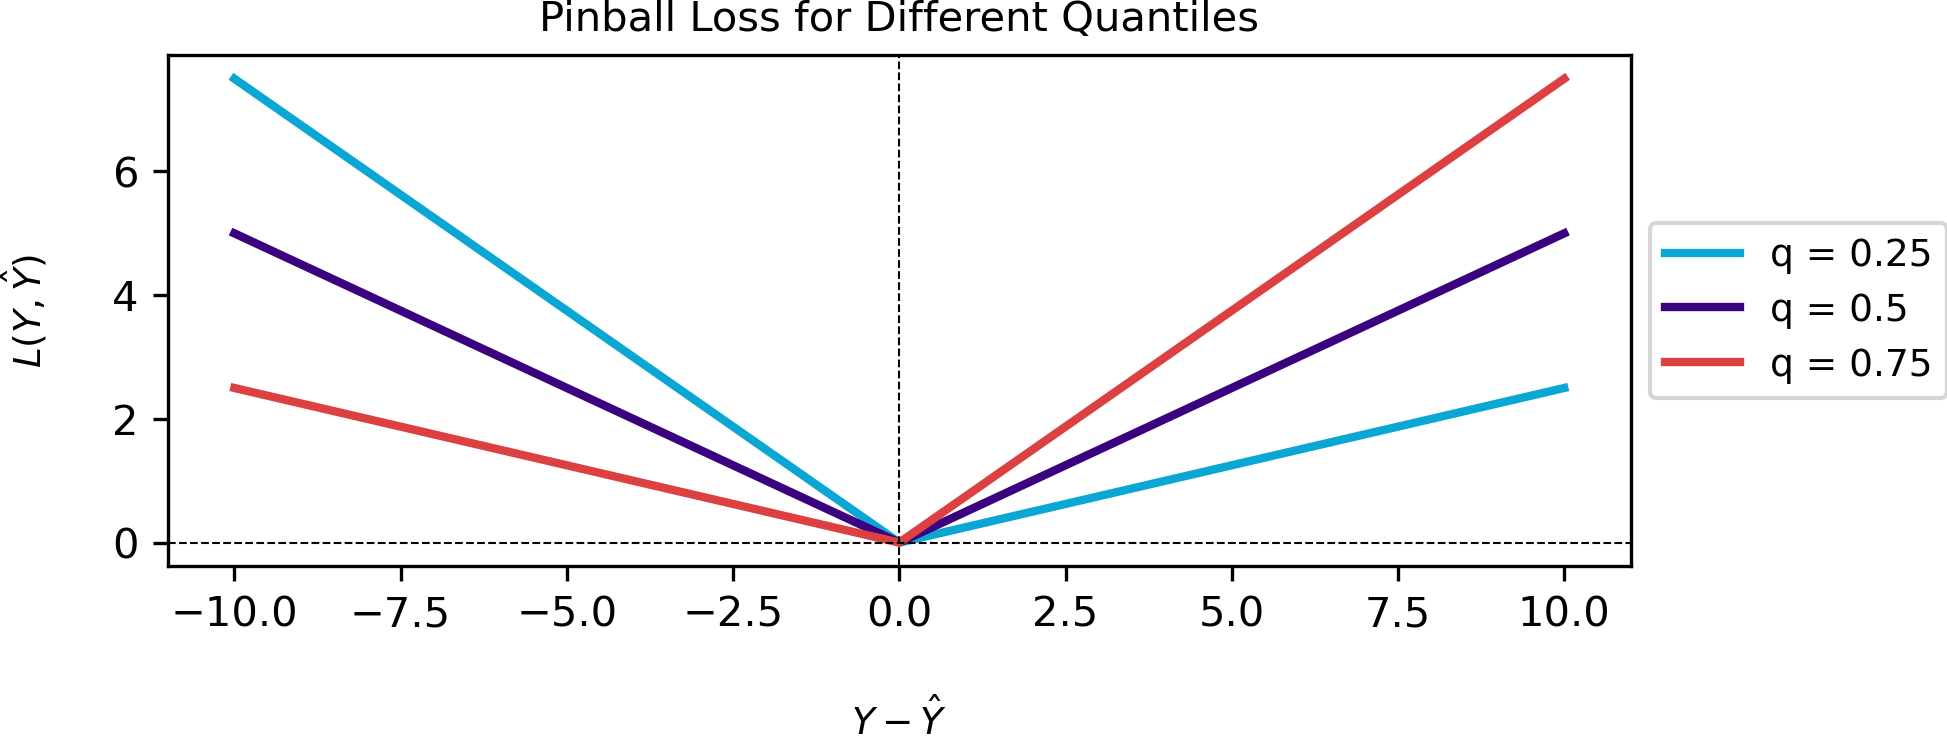
\includegraphics[width=0.40\textwidth]{figures/Pinball_Loss.png} 
    \vspace{-10pt} 
\end{wrapfigure}


\textbf{Figure 3.15 Pinball Loss.} Demonstrates the behavior of the Pinball Loss function for three different quantile values $(q = 0.25, 0.5, 0.75)$.
The plot shows how the loss increases linearly with the difference between the predicted value $\hat{Y}$ and the actual value $Y$ for various quantiles, with the loss function being asymmetric around the prediction.

\orangebox{Did you know that...}
{Pinball Loss is also called Quantile Loss and is an L1 Loss when $q=0.5$.}

% ---------- Explained Variance Score ----------
\clearpage
\thispagestyle{regressionstyle}
\section{Explained Variance Score}
\subsection{Explained Variance Score}

The Explained Variance Score (EVS) is a regression evaluation metric that measures the proportion of variance in the target variable that is captured by the model’s predictions.
It focuses specifically on how well the variability of the data is explained, rather than penalizing systematic biases or a lack of correlation between true and predicted values.

% formula
\begin{center}
    \tikz{
        \node[inner sep=2pt, font=\Large] (a) {
            {
                $\displaystyle
                EVS = 1 - \frac{Var({\color{nmlcyan}Y} - {\color{nmlpurple}\hat{Y}})}{Var({\color{nmlcyan}Y})}
                $
            }
        };
        
        \draw[-latex,nmlcyan, semithick] ($(a.north)+(1.2,0)$) to[bend right=15] node[pos=1, left] {actual value} +(-1,.5);
        \draw[-latex,nmlpurple, semithick] ($(a.north)+(2.3,0)$) to[bend left=15] node[pos=1, right] {predicted value} +(1,.5); 
    }
\end{center}

Explained Variance Score ranges from -infinity to 1, with 1 indicating that the model explains all variability in the target variable. Negative values suggest the model performs worse
than a horizontal line.

\textbf{Whent to use Explained Variance Score?}

When we need to wnderstanding how well the model explains the variability in the data.

\coloredboxes{
    \item Provides an intuitive measure of how much of the variance in the data is captured by the model.
}
{
    \item Explained Variance Score does not account for systematic offsets between predicted and true values, e.g., the explained variance score between 
    \( y=[1, 2, 3, 4] \) and \( \hat{y}=[8, 9, 10, 11] \). is equal to $1$ despite the predictions being off.
}

\chapter{Classification}

% ---------- Confusion Matrix ----------
\thispagestyle{classificationstyle}
\section{Confusion Matrix}
A confusion matrix is a table that shows how well a classification model makes predictions.
It compares the model's predicted labels with the true labels.

\vspace{-0.5em}
\begin{center}
\tikz{
\node[inner sep=2pt, font=\Large] (a) {
$\displaystyle
C_{\textcolor{nmlred}{i}\,\textcolor{nmlcyan}{j}}
= \sum_{n=1}^{M} 
\mathbf{1}\{ \; y_n = \textcolor{nmlred}{i} \;\land\; \hat{y}_n = \textcolor{nmlcyan}{j} \;\}
$
};
\draw[-latex,nmlred, semithick] ($(a.north west)+(6.2,0)$)
 to[bend left=15] node[pos=1, left] {Actual class $i$} +(-.5,.3);
\draw[-latex,nmlcyan, semithick] ($(a.north east)+(-.2,0)$)
 to[bend left=15] node[pos=1, right] {Predicted class $j$} +(.5,.3);
}
\end{center}
\vspace{-0.5em}


A simple 2x2 example for binary classification with four categories: True Positive (TP), True Negatives (TN), False Positive (FP), False Negative (FN).

\newcolumntype{C}[1]{>{\centering\arraybackslash}m{#1}}
\vspace{0.3em}
\begin{minipage}{0.46\linewidth}
\centering
\begin{tabular}{|C{1.4cm}|C{1.4cm}|}
\hline
Actual & Predicted \\ \hline
1 & 1 \\
1 & 0 \\
0 & 1 \\
0 & 0 \\
1 & 1 \\
0 & 0 \\
\hline
\end{tabular}
\end{minipage}%
\begin{minipage}{0.54\linewidth}
\renewcommand{\arraystretch}{1.8}
\centering
\begin{tabular}{|C{1.8cm}|C{1.8cm}|C{1.8cm}|}
\hline
& Predicted 1 & Predicted 0 \\ \hline
Actual 1 & \cellcolor{nmlgreen!20}TP = 2 & \cellcolor{nmlred!20}FP = 1 \\ \hline
Actual 0 & \cellcolor{nmlred!20}FN = 1 & \cellcolor{nmlgreen!20}TN = 2 \\ \hline
\end{tabular}
\end{minipage}

\vspace{0.8em}
\textbf{When to use Confusion Matrix?}

Use a confusion matrix whenever you are dealing with a classification task.
It is the fundamental tool from which most other performance metrics are derived,
making it unavoidable if you need to calculate precision, recall, F1-score, or other related measures.

\vspace{0.3em}
\coloredboxes{
\item Provides a detailed breakdown of correct and incorrect classifications.
\item Forms the foundation for many key performance metrics (e.g., precision, recall, F1).
\item Works for both binary and multi-class classification.
}
{
\item Can become large and harder to interpret for problems with many classes.
\item Does not directly provide a single performance score (requires additional derived metrics).
\item Sensitive to class imbalance; raw counts may be misleading without normalization.
}
\clearpage
In some interesting real-world industries, it is difficult to construct a standard confusion matrix. 

For instance, in predictive maintenance, machine learning models predict when a machine might fail so maintenance can be scheduled in advance.

If the model predicts a breakdown and maintenance is performed, the machine may never actually fail. This means the usual true positives (TP) are no longer observable.

This raises the question: How can we be sure the model was correct? Is there a way to know whether or not our machine would have failed if we had not maintained it?
This lack of failure is our original goal, and it is beneficial. However, it also results in no immediate failure or target data to validate the model’s prediction. 
The critical feedback is delayed, and the resultant confusion matrix is “censored”.

\newcolumntype{C}[1]{>{\centering\arraybackslash}m{#1}}
\begin{table}[h]
\centering
\renewcommand{\arraystretch}{2.5}
\begin{tabular}{|C{2cm}|C{2cm}|C{2cm}|C{2cm}|}
\hline
& \multicolumn{3}{c|}{\textbf{Model predicts machine failure}} \\
\cline{2-4}
X & Total Population (P+N)& 
Positive & 
Negative \\
\hline
\multirow{2}{2cm}{\textbf{Does Machine fail in Reality?}} & 
Positive & 
Not available  & 
Delayed \\
\cline{2-4}
& 
Negative & 
Not available & 
Delayed \\
\hline
\end{tabular}
\end{table}


\orangebox{%
Did you know that...}
{It is also known as error matrix typically in a supervised learning usecase; in unsupervised learning it is usually called a matching matrix. 
}

\textbf{Other related metrics}
Metrics that one can derive from confusion matrix like accuracy, precision, recall and more. 




% ---------- FPR ----------
\clearpage
\section{FPR}
\subsection{False Positive Rate}
\thispagestyle{classificationstyle}

The False Positive Rate (FPR), also known as the false alarm ratio or fall-out, measures how often negative instances are incorrectly classified as positive in binary classification.

\begin{center}
\tikz{
\node[inner sep=2pt, font=\Large] (a) {
{
$\displaystyle
FPR = \frac{{\color{cyan}FP}}{{\color{cyan}FP} + {{\color{nmlpurple}TN}}}
$
}
};
\draw[-latex,cyan, semithick] ($(a.north)+(1.3,0.05)$) to[bend left=15] node[pos=1, right] {False positives} +(1,.5); 
% \draw[-latex,teal!70!green, semithick] ($(a.south)+(2.1,0.1)$) to[bend right=15] node[pos=1, right] {Mean of targets} +(1,-.5); 
\draw[-latex,nmlpurple, semithick] ($(a.south)+(1.5,-0.05)$) to[bend left=15] node[pos=1, left] {True negatives} +(-1,-.5); 
}
\end{center}

FPR ranges from 0 (no false alarms) to 1 (all predicted positives are incorrect). FPR can also be interpreted as the probability that a negative instance will be incorrectly identified as positive.

\textbf{When to use FPR?}

Use FPR when you need to evaluate how well a classifier avoids false positives, especially when false positives have significant costs, like in medical diagnostics or security systems. It's also useful for understanding the trade-off between true positive rate (sensitivity) and false positive rate.

\coloredboxes{
\item It provides a clear and intuitive measure of a classifier's false positive performance.
\item It helps identify scenarios where the classifier is overly sensitive and prone to false alarms.
}
{
\item FPR does not consider true positive instances.
\item FPR can be sensitive to class imbalance, as it may be easier to achieve a low FPR when the negative class is dominant.
\item FPR doesn't exist in isolation; it's often important to show its relationship with another key metric. (e.g., TPR, Precision, Recall).
}


\clearpage
\thispagestyle{customstyle}


\begin{figure*}[ht!]
    \centering
    \includegraphics[width=0.7\textwidth]{figures/FPR_3d_surface.png}
    % \caption{Caption}
    \label{fig1}
\end{figure*}

\begin{wrapfigure}{r}{0.55\textwidth}
    \centering
    \vspace{-20pt} % Adjust vertical alignment if needed
    \includegraphics[width=0.5\textwidth]{figures/FPR_2d_line_plot.png} % Your figure goes here
\end{wrapfigure}

% Left text with the image on the right
\textbf{Figure 3.1 False Positive Rate.} 
\textbf{Top:}
3D surface illustrating FPR's non-linear relationship with FP and TN. FPR is lowest (blue) when FP is low. It increases (red) as FP increases.
\textbf{Right:}
Shows how FPR decreases hyperbolically as total negative cases increase for fixed FP values. Lower FP maintains better FPR.


\orangebox{%
Did you know that...}
{
In the context of statistical hypothesis testing, the FPR is also known as the "type I error rate" or the probability of rejecting a true null hypothesis.
}

\textbf{Other related metrics}

Other metrics used alongside or instead of FPR include True Positive Rate (TPR), Precision, F1-Score, Receiver Operating Characteristic (ROC AUC), and Specificity.


% ---------- FNR ----------
\clearpage
\section{FNR}
\subsection{False Negative Rate}
\thispagestyle{classificationstyle}

The False Negative Rate (FNR), also known as the miss rate, measures the proportion of actual positive instances incorrectly classified as negative in binary classification.
\begin{center}
\tikz{
\node[inner sep=2pt, font=\Large] (a) {
{
$\displaystyle
FNR = \frac{{\color{cyan}FN}}{{\color{cyan}FN} + {{\color{nmlpurple}TP}}}
$
}
};
\draw[-latex,cyan, semithick] ($(a.north)+(1.3,0.05)$) to[bend left=15] node[pos=1, right] {False negatives} +(1,.5); 
% \draw[-latex,teal!70!green, semithick] ($(a.south)+(2.1,0.1)$) to[bend right=15] node[pos=1, right] {Mean of targets} +(1,-.5); 
\draw[-latex,nmlpurple, semithick] ($(a.south)+(1.5,-0.05)$) to[bend left=15] node[pos=1, left] {True positives} +(-1,-.5); 
}
\end{center}

FNR ranges from 0 (no false negatives) to 1 (all positive instances misclassified). It represents the probability that a positive instance will be incorrectly identified as negative.

\textbf{When to use FNR?}

Use FNR when the cost of missing positive cases is high (e.g., in medical diagnostics or fraud detection) or when you must balance false negatives and false positives.

\coloredboxes{
\item It directly measures the rate of missed positive cases.
\item It is critical in fields where false negatives have severe consequences.
\item Complements True Positive Rate (TPR) in assessing classifier performance.
}
{
\item It doesn't account for true negatives or false positives.
\item It can be misleading in highly imbalanced datasets.
\item It should be considered alongside other metrics for a comprehensive evaluation.
}


\clearpage
\thispagestyle{customstyle}


\begin{figure*}[ht!]
    \centering
    \includegraphics[width=0.7\textwidth]{figures/FNR_3d_surface.png}
    % \caption{Caption}
\end{figure*}

\begin{wrapfigure}{r}{0.55\textwidth}
    \centering
    \vspace{-20pt} % Adjust vertical alignment if needed
    \includegraphics[width=0.5\textwidth]{figures/FNR_2d_line_plot.png} % Your figure goes here
\end{wrapfigure}

% Left text with the image on the right
\textbf{Figure 3.1 False Negative Rate.} 
\textbf{Top:}
3D surface illustrating FNR's non-linear relationship with FN and TP. FNR is lowest (blue) when FN is low. It increases (red) as FN increases.
\textbf{Right:}
Shows how FNR decreases hyperbolically as total positive cases increase for fixed FN values. Lower FN maintains better FNR.


\orangebox{%
Did you know that...}
{
    In hypothesis testing, reducing the False Negative Rate ($\beta$) increases the power of the test ($1 - \beta$), but often at the cost of increasing the False Positive Rate ($\alpha$).
    This demonstrates the inherent trade-off between Type I and Type II errors in statistical testing.
}

\textbf{Other related metrics}

Other metrics used alongside or instead of False Negative Rate
are Recall/Sensitivity, Specificity, Precision, F1-Score, and ROC curve.

% ---------- TPR ----------
\clearpage
\section{TPR (Recall/Sensitivity)}
\subsection{True Positive Rate (Recall/Sensitivity)}
\thispagestyle{classificationstyle}

Recall, also known as Sensitivity or True Positive Rate (TPR), is a crucial metric in classification tasks. It measures the proportion of actual
positive instances that were correctly identified by the model. Recall answers the question: "Of all the positive cases, how many did our model correctly identify?”

\begin{center}
\tikz{
\node[inner sep=2pt, font=\Large] (a) {
{
$\displaystyle
Recall = \frac{{\color{cyan}TP}}{{\color{cyan}TP} + {{\color{nmlpurple}FN}}}
$
}
};
\draw[-latex,cyan, semithick] ($(a.north)+(1.3,0.05)$) to[bend left=15] node[pos=1, right] {True positives} +(1,.5); 
% \draw[-latex,teal!70!green, semithick] ($(a.south)+(2.1,0.1)$) to[bend right=15] node[pos=1, right] {Mean of targets} +(1,-.5); 
\draw[-latex,nmlpurple, semithick] ($(a.south)+(1.5,-0.05)$) to[bend left=15] node[pos=1, left] {False negatives} +(-1,-.5); 
}
\end{center}

Recall ranges from 0 to 1, where 1 indicates perfect recall (all positive instances were correctly identified), and 0 indicates the worst
possible recall (no positive instances were identified).

\textbf{When to use Recall?}
When the cost of false negatives is high (e.g., missing a fraudulent transaction or a critical medical diagnosis).
When you need to identify as many positive instances as possible, even at the risk of some false positives. In imbalanced datasets where the positive class is rare but important.

\coloredboxes{
\item Focuses on minimizing false negatives, which is crucial in many high-stakes applications.
\item Provides insight into a model's ability to find all positive instances.
\item Useful in scenarios where missing a positive is more costly than incorrectly labeling a negative
}
{
\item Doesn't account for false positives, which can lead to high recall but poor precision.
\item Can be misleading when used in isolation, as a model that predicts everything as positive would have perfect recall.
\item Ignores performance on negative examples, which may be important in some contexts.
}


\clearpage
\thispagestyle{customstyle}


\begin{figure*}[ht!]
    \centering
    \includegraphics[width=0.7\textwidth]{figures/Recall_3d_surface.png}
    % \caption{Caption}
\end{figure*}

\begin{wrapfigure}{r}{0.55\textwidth}
    \centering
    \vspace{-20pt} % Adjust vertical alignment if needed
    \includegraphics[width=0.5\textwidth]{figures/Recall_2d_line_plot.png} % Your figure goes here
\end{wrapfigure}

% Left text with the image on the right
\textbf{Figure 3.5 Recall.} 
\underline{Top:}
Shows how Recall decreases hyperbolically as total positive cases increase for fixed TP values. Higher TP maintains better Recall.
Curves display a rapid initial decline followed by a gradual decrease.
\underline{Right:}
3D surface illustrating Recall's non-linear relationship with TP and FN. Recall is highest (blue) when TP is high and FN is low, decreasing (red) as FN increases or TP decreases.

\orangebox{%
Did you know that...}
{
    Precision and Recall were introduced by Allen Kent in the 1950s. These metrics were initially developed to evaluate the effectiveness of library catalog
    systems and early computerized document retrieval systems.
}

\textbf{Other related metrics}

Other metrics used alongside or instead of Recall are Precision, F1-Score, F-beta, Specificity, ROC AUC and, Matthews Correlation Coefficient (MCC).

% ---------- TNR ----------
\clearpage
\thispagestyle{classificationstyle}
\section{TNR (Specificity)}
\subsection{True Negative Rate (Specificity)}

True Negative Rate (TNR), also known as specificity, measures the proportion of actual negative instances correctly identified as such in binary classification.
Specificity is a crucial metric in evaluating diagnostic tests and classification models.

\begin{center}
    \tikz{
        \node[inner sep=2pt, font=\Large] (a) {
        {
        $\displaystyle
        TNR = \frac{{\color{cyan}TN}}{{\color{cyan}TN} + {{\color{nmlpurple}FP}}}
        $
        }
        };
        \draw[-latex,cyan, semithick] ($(a.north)+(1.3,0.05)$) to[bend left=15] node[pos=1, right] {True negatives} +(1,.5); 
        % \draw[-latex,teal!70!green, semithick] ($(a.south)+(2.1,0.1)$) to[bend right=15] node[pos=1, right] {Mean of targets} +(1,-.5); 
        \draw[-latex,nmlpurple, semithick] ($(a.south)+(1.5,-0.05)$) to[bend left=15] node[pos=1, left] {False positives} +(-1,-.5); 
    }
\end{center}

TNR ranges from 0 to 1, where 1 indicates perfect specificity (all negative instances correctly identified) and 0 (no negative instances were correctly identified).
In hypothesis testing, specificity is inversely related to the Type I error rate.

\textbf{Why to use TNR?}

When you need to assess a test's ability to identify negative cases correctly or when the cost of false positives is high (e.g., unnecessary medical procedures).

\coloredboxes{
\item It directly measures the ability to correctly identify negative cases.
\item It is crucial in scenarios where false positives have significant consequences.
\item High specificity is valuable for confirmatory tests.
}
{
\item It doesn't account for false negatives or true positives.
\item A test with high specificity but low sensitivity might miss many positive cases.
\item It should be considered alongside sensitivity for a comprehensive evaluation.
}

\clearpage
\thispagestyle{customstyle}

\orangebox{%
Did you know that...}
{
    Sensitivity and Specificity were introduced by the American biostatistician Jacob Yerushalmy in 1947.
}

\textbf{Other related metrics}

Other metrics used alongside or instead of TNR include TPR (Sensitivity/Recall). FPR, which is 1 - Specificity, F1-Score, and ROC curve.

% ---------- Accuracy ----------
\clearpage

\thispagestyle{classificationstyle}
\section{Accuracy}
\subsection{Accuracy} 

Accuracy is a frequently used classification metric as it provides an intuitive answer to the question, "How often is the classifier correct?”.
Accuracy measures a model's overall correctness across all classes by calculating the proportion of correct predictions among the total number of cases examined.

% formula
\begin{center}
    \tikz{
        \node[inner sep=2pt, font=\Large] (a) {
            {
                $\displaystyle
                Accuracy = \frac{{\color{nmlred}TP}+{\color{cyan}TN}}{{\color{nmlred}TP} + {{\color{cyan}TN}} + {\color{nmlpurple}FP} + {\color{teal!70!green}FN}}
                $
            }
        };
        \draw[-latex, cyan, semithick] ($(a.north)+(2, 0.05)$) to[bend left=15] node[pos=1, right] {True negatives} +(1,.5); 
        \draw[-latex, nmlpurple, semithick] ($(a.south)+(2, -0.05)$) to[bend left=15] node[pos=1, left] {False positives} +(-1,-.5);
        \draw[-latex, nmlred, semithick] ($(a.north)+(0.7, 0.05)$) to[bend right=20] node[pos=1, left] {True positives} +(-1,.5);
        \draw[-latex, teal!70!green, semithick] ($(a.south)+(3.5,-0.05)$) to[bend right=15] node[pos=1, right] {False negatives} +(1,-.5);
    }
\end{center}

Accuracy ranges from 0 to 1, with 1 representing perfect classification. While accuracy may be easy to understand, it can be misleading when dealing with imbalanced datasets.
It is best used when the classes in the dataset are roughly balanced, and all misclassification errors are equally costly.

\textbf{When to use Accuracy?}

Use accuracy when you need a simple, interpretable metric and your dataset is balanced. Avoid using it as the sole metric for imbalanced datasets or when different errors have varying costs.

\coloredboxes{
\item Accuracy provides an easily understandable measure of model performance.
\item It works well for balanced datasets where all classes are equally important.
}
{
\item Accuracy can be misleading for imbalanced datasets, potentially hiding poor performance in minority classes.
\item It doesn't distinguish between different types of errors (false positives vs. false negatives).
}

% ---------- Balanced Accuracy ----------
\clearpage
\thispagestyle{classificationstyle}
\section{Balanced Accuracy}
\subsection{Balanced Accuracy}

Balanced Accuracy is a classification evaluation metric that accounts for class imbalance. In binary classification it can be undertood as the arithmetic mean between
specificity and sensitivity (recall). In multi-class classification Balanced Accuracy is the average of the recall obtained in each class, i.e. the macro-average of recall scores per class.

% formula
\begin{center}
    [FORMULA GOES HERE]
\end{center}

It is particularly useful when working with datasets where some classes are significantly underrepresented, ensuring that the performance of all classes is treated equally.
The score ranges from 0 to 1. If the dataset is balance, then Balanced Accuracy score reduces to the conventional Accuracy.

\textbf{When to use Balanced Accuracy?}

When dealing with class imbalance. Balanced Accuracy ensures that underrepresented classes are not overshadowed by majority classes in the performance metric.

\coloredboxes{
\item Unlike standard accuracy, it gives equal importance to all classes, making it more reliable for imbalanced datasets.
\item Provides an intuitive measure of how well the model performs across all classes.
}
{
\item Treats all classes equally, which may not be ideal if some classes are more critical than others.
\item Under extreme class imbalance or small sample sizes, balanced accuracy can show high variance, as the performance of the minority class has a strong impact on the overall score.
}

% ---------- Precision ----------
\clearpage
\thispagestyle{classificationstyle}
\section{Precision}
\subsection{Precision}

Precision measures the accuracy of positive predictions made by a classifier. It is the ratio of correctly predicted positive instances (true positives) to
the total number of instances predicted as positive (true positives + false positives). It answers the question: “Out of all the cases indicated as positive, how many are as actual positives?”

% formula
\begin{center}
    \tikz{
        \node[inner sep=2pt, font=\Large] (a) {
            {
                $\displaystyle
                Precision = \frac{{\color{nmlcyan}TP}}{{\color{nmlcyan}TP} + {\color{nmlpurple}FP}}
                $
            }
        };
        \draw[-latex, nmlcyan, semithick] ($(a.north)+(1.4, 0.05)$) to[bend left=15] node[pos=1, right] {True positives} +(1,.5); 
        \draw[-latex, nmlpurple, semithick] ($(a.south)+(2, -0.05)$) to[bend left=15] node[pos=1, left] {False positives} +(-1,-.5);
    }
\end{center}

Precision ranges from 0 to 1, where 1 indicates perfect precision (all predicted positives are correct), and 0 indicates the worst performance (no predicted positives are correct).

\textbf{When to use Precision?}

Precision is important when the cost of false positives is high. For example, in spam detection, you don’t want legitimate emails ending up in the spam folder,
and in recommendation systems, irrelevant suggestions (false positives) can frustrate users.

\coloredboxes{
\item Focuses on the accuracy of positive predictions.
\item Critical in applications where false positives are costly or disruptive.
}
{
\item Doesn't account for false negatives, which can lead to high precision but poor recall.
\item It can be misleading when used in isolation, as a model that predicts only one sample as positive and correctly gets it would have perfect precision.
}

\orangebox{%
Did you know that...}
{
    Precision and Recall often have an inverse relationship. As you increase Precision, Recall tends to decrease, and vice versa.
    This is known as the Precision-Recall trade-off curve.
}

% ---------- F1-score ----------
\clearpage
\thispagestyle{classificationstyle}
\section{F1-score}
\subsection{F1-score}

The F1 score or balanced F-score measures a classifier's predictive performance by assessing classes' performance. We can think of the F1-score as the harmonic mean of the model’s
precision and recall, thus giving equal weight to both these metrics. So, the F1-score is critical when we care equally about avoiding false positives
(e.g., incorrectly marking an important email as spam) and false negatives (e.g., missing a spam email).


% formula
\begin{center}
    \tikz{
        \node[inner sep=2pt, font=\Large] (a) {
            {
                $\displaystyle
                F1 = \frac{2}{\textcolor{nmlcyan}{P^{-1}} + \textcolor{nmlpurple}{R^{-1}}} = \frac{2\textcolor{nmlred}{TP}}{2\textcolor{nmlred}{TP} + \textcolor{nmlgreen}{FP} + \textcolor{gray}{FN}}
                $
            }
        };
    \draw[-latex, nmlcyan, semithick] ($(a.south)+(-2.7, -0.05)$) to[bend left=25] node[pos=1, left] {\color{nmlcyan} precision} +(-.6, -.5);
    \draw[-latex, nmlpurple, semithick] ($(a.south)+(-1.2, -0.05)$) to[bend left=-35] node[pos=1, right] {\color{nmlpurple} recall} +(0.7, -.9);
    \draw[-latex, nmlgreen, semithick] ($(a.south)+(2.3, -0.05)$) to[bend left=35] node[pos=1, left] {\color{nmlgreen} false positive} +(-0.5, -.4);
    \draw[-latex, gray, semithick] ($(a.south)+(3.4, -0.05)$) to[bend left=-30] node[pos=1, right] {\color{gray} false negative} +(0.7, -.6);
    \draw[-latex, nmlred, semithick] ($(a.south)+(2.3, 1.3)$) to[bend right=-40] node[pos=1, right] {\color{nmlred} true positive} +(0.7, .6);
    }
\end{center}

The F1-score ranges from 0 to 1. Maximizing precision and recall allows us to approximate a perfect classifier. However, bear in mind that in practice, there is a
trade-off between precision and recall, so improving precision may inadvertently decrease recall and vice versa.

\textbf{When to use Accuracy?}

Use the F1-score when you need a balanced measure of a model's performance, with an equal balance between precision and recall (when false positives and negatives are concerns).

\coloredboxes{
\item F1-score provides a single, easy-to-interpret metric that equally weights precision and recall.
\item It works better than accuracy for imbalanced datasets.
}
{
\item The F1-score doesn't consider true negatives, which might be necessary in some scenarios.
\item It assumes that precision and recall are equally important. F-beta score can address this by allowing adjustable weighting between precision and recall.
}

% ---------- F-beta ----------
\clearpage
\thispagestyle{classificationstyle}
\section{F-beta}
\subsection{F-beta}

The F-beta Score is a classification evaluation metric that balances the trade-off between precision and recall, allowing us to give different levels of importance to each.
It is an extension of the F1-score, where the parameter  determines the weight of recall relative to precision.

% formula
\begin{center}
    \tikz{
        \node[inner sep=2pt, font=\Large] (a) {
        {
            $\displaystyle
            F_{\beta} = \frac{(1 + \beta^2) {\color{nmlred}TP}}{(1 + \beta^2) {\color{nmlred}TP} + {\color{nmlpurple}FP} + \beta^2 {\color{teal!70!green}FN}} = \frac{(1 + \beta^2) \cdot {\color{nmlcyan}P} \cdot {\color{nmlyellow}R}}{\beta^2 \cdot {\color{nmlcyan}P} + {\color{nmlyellow}R}}
            $
        }
        };
        \draw[-latex, nmlred, semithick] ($(a.north)+(-0.5, 0.05)$) to[bend right=20] node[pos=1, left] {True positives} +(-1,.5);
        \draw[-latex, nmlcyan, semithick] ($(a.north)+(4.6,0.05)$) -- +(0,0.65) node[above, yshift=2pt] {Precision};
        \draw[-latex, nmlpurple, semithick] ($(a.south)+(-0.8, -0.05)$) to[bend left=15] node[pos=1, left] {False positives} +(-1,-.5);
        \draw[-latex, teal!70!green, semithick] ($(a.south)+(1.2,-0.05)$) -- +(0,-0.6) node[below, yshift=-2pt] {False negatives};
        \draw[-latex, nmlyellow, semithick] ($(a.south)+(4.8,-0.05)$) -- +(0,-0.6) node[below, yshift=-2pt] {Recall};
    }
\end{center}

Similar to the F1-score, the highest possible value is 1.0, indicating perfect precision and recall, while the lowest possible value is 0, which occurs when both precision and recall are zero.
The two most common $\beta$ values are 2, which weights recall higher than precision, and 0.5, which, conversely, weights precision higher than recall.

\textbf{When to use F-beta?}

The F-beta Score is particularly useful when Precision and Recall are unequally important.

\coloredboxes{
\item F-beta is customizable. It allows to prioritize precision or recall based on the context of your problem.
\item Helps balancing the trade-off between precision and recall.
}
{
\item Choosing an appropriate value for $\beta$ can be non-trivial and requires domain knowledge.
\item Just like F1-score, F-beta doesn't consider true negatives, which might be necessary in some scenarios.
}

% ---------- ROC AUC ----------
\clearpage
\thispagestyle{classificationstyle}
\section{ROC AUC}
\subsection{Area Under the Receiver Operating Characteristic Curve}

The Receiver Operating Characteristic (ROC) plot illustrates a classifier's performance at different thresholds. The curve help us undertand the trade-off between FPR
and TPR at different thresholds. ROC curves can be summarized in a single value by calculating their area under the curve (AUC), which ranges from 0 to 1.0.
Given one randomly selected positive instance and one randomly chosen negative example, the AUC is the probability that the classifier will be able to tell which is which.

% formula
\begin{center}
    \tikz{
        \node[inner sep=2pt, font=\Large] (a) {
        {
            $\displaystyle
            \begin{aligned}
            ROC-AUC &= \int_{{\color{nmlgreen}0}}^{{\color{nmlgreen}1}} ROC({\color{nmlgreen}T}) \, d{\color{nmlgreen}T} \\[2em]
                    &= \int_{0}^{1} {\color{nmlpurple}TPR}({\color{nmlcyan}FPR}^{-1}(x)) \, dx
            \end{aligned}
            $
        }
        };
        \draw[-latex, nmlgreen, semithick] ($(a.north)+(1.5,-0.3)$) to[bend left=15] node[pos=1, right] {Threshold} +(1,.9);
        \draw[-latex, nmlpurple, semithick] ($(a.south)+(0.5,1.1)$) to[bend left=15] node[pos=1, right] {True Positive Rate} +(1,.9);
        \draw[-latex, nmlcyan, semithick] ($(a.south)+(1.9,0.25)$) to[bend right=15] node[pos=1, right] {False Positive Rate} +(1,-.9);
    }
\end{center}

A common misconception is that a model with an AUC of 0.5 implies that the classifier is no better than random guessing. This misconception is a "fallacy of the undistributed middle":
all random models score an AUC of 0.5, but not every model that scores an AUC of 0.5 is random.

\textbf{When to use ROC AUC?}

ROC AUC is ideal when you need a threshold-independent measure to evaluate and compare different classifiers across various operating points. It's especially helpful when the costs of
false positives and false negatives are unknown or equally important.

\clearpage
\coloredboxes{
\item ROC AUC is threshold-independent. It summarizes classifier performance across all possible thresholds.
\item It allows for a probabilistic interpretation, providing a clear comparison between different models.
}
{
\item It can be misleading if the goal is to optimize performance at a specific threshold. Models can have the same AUC but vary in performance at key thresholds.
\item It summarises performance over regions of the ROC space in which one would rarely operate, such as extreme right (high FPR) or extreme left side (low TPR).
\item ROC AUC doesn't inform about precision and negative predicted value.
}

% ---------- PR AUC ----------
\clearpage
\thispagestyle{classificationstyle}
\section{PR AUC}
\subsection{Area Under the Precision-Recall Curve}

The Precision-Recall (PR) curve focuses on the trade-off between precision (positive predictive value) and recall (true positive rate) across various thresholds.
Precision measures how many of the predicted positives are actually positive, while recall captures how many actual positives were identified.
The PR AUC represents the area under this curve, offering a single-value summary of a model's performance.

% formula
\begin{center}
    \tikz{
        \node[inner sep=2pt, font=\Large] (a) {
        {
            $\displaystyle
            PR-AUC = \int_{{\color{nmlyellow}0}}^{{\color{nmlyellow}1}} {\color{nmlcyan}P}({\color{nmlyellow}R}) \, d{\color{nmlyellow}R}
            $
        }
        };
        \draw[-latex, nmlcyan, semithick] ($(a.north)+(1.3, -0.3)$) to[bend right=20] node[pos=1, left] {Precision} +(-1,.9);
        \draw[-latex, nmlyellow, semithick] ($(a.north)+(1.9,-0.3)$) to[bend left=15] node[pos=1, right] {Recall} +(1,.9);
    }
\end{center}

Similar to the F1-score, the highest possible value for PR AUC is 1.0, indicating perfect precision and recall, while the lowest possible value is 0.
The main difference between PR AUC and ROC AUC is how they treat true negatives. PR AUC doesn't consider true negatives, which is why it is preferred over ROC AUC
when true negatives are not relevant to the problem.

\textbf{When to use PR AUC?}

Similarly to ROC AUC, PR AUC is ideal when you need a threshold-independent measure to evaluate and compare different classifiers across various operating points. 
It is particularly useful in imbalanced datasets, where one class (typically the positive class) is much rarer than the other. In such cases, PR AUC provides a more
informative measure of a model's ability to detect the minority class without being overly influenced by the majority class.

\coloredboxes{
\item PR AUC highlights performance on the minority class, making it invaluable for imbalanced datasets.
}
{
\item PR AUC doesn't provide insights into the true negative predictions.
\item It summarises performance over regions of the PR space in which one would rarely operate.
}


% ---------- Brier Score Loss ----------
\clearpage
\thispagestyle{classificationstyle}
\section{Brier Score Loss}
\subsection{Brier Score Loss}

The Brier Score Loss is a metric used to evaluate the accuracy of predicted probabilities in binary classification problems.
It calculates the mean squared error between the predicted probabilities and the actual binary outcomes, providing a measure of how well-calibrated the predictions are.

% formula
\begin{center}
    \tikz{
        \node[inner sep=2pt, font=\Large] (a) {
        {
            $\displaystyle
            {Brier\ Score} = \frac{1}{{\color{nmlred}N}} \sum_{i=1}^{N} ({\color{nmlpurple}y_i} - {\color{nmlcyan}p_i})^2
            $
        }
        };
        \draw[-latex, nmlpurple, semithick] ($(a.north)+(1.7, -0.5)$) to[bend right=20] node[pos=1, left] {Actual outcome} +(-1,.9);
        \draw[-latex, nmlcyan, semithick] ($(a.south)+(2.7,0.5)$) to[bend right=15] node[pos=1, right] {Predicted probability} +(1,-.5);
        \draw[-latex, nmlred, semithick] ($(a.south)+(0.2,0.1)$) to[bend left=15] node[pos=1, left] {Number of samples} +(-1,-.5);
    }
\end{center}

The Brier Score ranges from 0 to 1, where 0 indicates perfect probabilistic predictions, and 1 means worst possible predictions. Because of its similarity with the MSE,
which can be decomposed as the sum of the variance and the squared of the bias. The Brier Score Loss can be decomposed as the sum of calibration loss and refinement loss.
For multi-class classification, the Brier Score can be extended to: ${Brier\ Score} = \frac{1}{N} \sum_{i=1}^{N} \sum_{j=1}^{C} (y_{ij} - p_{ij})^2$ where $C > 2$ is the number of classes.


\textbf{When to use the Brier Score Loss?}

When probability calibration is as important as the classification accuracy. Like when the problem requires reliable probability estimates for downstream tasks
like risk assessment or decision-making.

\coloredboxes{
\item Summarices both predictive accuracy and calibration in one value.
}
{
\item Only suitable for binary tasks. It is inappropriate for ordinal variables which can take three or more values.
}

% ---------- Log Loss ----------
\clearpage
\thispagestyle{classificationstyle}
\section{Log Loss}
\subsection{Log Loss}

The Log Loss, also known as cross-entropy loss or logistic regression loss is a classification metric that evaluates the accuracy of predicted probabilities by
penalizing predictions that are both incorrect and overly confident. It measures the distance between the predicted probabilities and the actual class labels.

% formula
\begin{center}
    \tikz{
        \node[inner sep=2pt, font=\Large] (a) {
        {
            $\displaystyle
            {Log\ Loss} = -\frac{1}{{\color{nmlred}N}} \sum_{i=1}^{N} ({\color{nmlpurple}y_i} \cdot log({\color{nmlcyan}p_i}) + (1 - {\color{nmlpurple}y_i}) \cdot log(1 - {\color{nmlcyan}p_i}))
            $
        }
        };
        \draw[-latex, nmlpurple, semithick] ($(a.north)+(-1.3, -0.5)$) to[bend right=20] node[pos=1, left] {Actual outcome} +(-1,.9);
        \draw[-latex, nmlcyan, semithick] ($(a.north)+(0.4,-0.5)$) to[bend left=15] node[pos=1, right] {Predicted probability} +(1,.9); 
        \draw[-latex, nmlred, semithick] ($(a.south)+(-2.6,0.25)$) to[bend right=15] node[pos=1, right] {Number of samples} +(1,-.9);
    }
\end{center}

As is common with loss metrics, smaller values are better. Log Loss ranges from 0 to infinity, where 0 indicates perfect probabilistic predictions and higher values
represent worse predictions. The formula above defines Log Loss for binary classification, but it can also be extended to multiclass classification:  
$Log Loss = -\frac{1}{N} \sum_{i=1}^{N} \sum_{j=1}^{C} y_{ij} log(p_{ij})$.
One key difference between Log Loss and Brier Score is that Log Loss is more sensitive to differences in predicted probabilities. This can be either an advantage or a
disadvantage, depending on the use case.


\textbf{When to use Log Loss?}

When you want to evaluate both the accuracy and confidence of predicted probabilities. Similar to the Brier Score, Log Loss is also useful when calibration
and well-distributed probabilities are important for downstream tasks such as ranking or risk assessment.

\coloredboxes{
    \item It is also a proper loss function, commonly used in logistic regression and neural networks.
    \item Generalizable beyond binary classification.
}
{
    \item Predictions close to 0 or 1 for the wrong class can heavily increase the loss.
    \item Not suitable if the model doesn't output well-calibrated probabilities.
}

% ---------- Jaccard Index ----------
\clearpage
\thispagestyle{classificationstyle}
\section{Jaccard Index}
\subsection{Jaccard Index}

The Jaccard Index, or Jaccard Similarity Coefficient, is a similarity metric often used for evaluating the performance of classification models,
particularly in segmentation tasks. It measures the overlap between the predicted set and the ground truth set.

\begin{center}
    \tikz{
        \node[inner sep=2pt, font=\Large] (a) {
            {
                $\displaystyle 
                J(A, B) = 
                \frac{\textcolor{nmlpurple}{|A \cap B|}}
                {\textcolor{nmlcyan}{|A \cup B|}}
                $
            }
        };
        \draw[-latex, nmlpurple, semithick] ($(a.south)+(1.2, 1.4)$) to[bend right=35] node[pos=1, left] {\color{nmlpurple} Intersection (common elements)} +(-0.9, .7);
        \draw[-latex, nmlcyan, semithick] ($(a.south)+(1.2,0.04)$) to[bend right=35] node[pos=1, right] {\color{nmlcyan} Union (all elements)} +(.9, -.7);
    }
\end{center}

The Jaccard Index ranges from 0 to 1, where 1 indicates perfect overlap between the predicted and true sets (i.e., all predictions are correct),
and 0 means no overlap at all. In binary classification, the formula can be rewritten in terms of true positives $TP$, false positives $FP$, and false negatives
$FN$ as: $J = \frac{TP}{TP + FP + FN}$. Additionally, the Jaccard Index is a popular metric for evaluating computer vision
models for image segmentation tasks, in those cases it is communly known as Intersection over Union (IoU).

\textbf{When to use the Jaccard Index}

It is particularly useful when we need to measure the similarity between two sets. For example, it can be used to assess the similarity between text documents,
evaluate preferences in recommender systems, or measure the similarity between genetic sequences.

\coloredboxes{
    \item Intuitive interpretation. It provides a straightforward measure of overlap, useful for visualization.
    \item Scale-Invariance. The Jaccard Index is not affected by the size of the sets being compared.
}
{
    \item Can be computationally expensive. Calculating the intersection and union for large or high dimensonal sets can be resource-intensive.
}


% ---------- D-squared Log Loss Score ----------
\clearpage
\thispagestyle{classificationstyle}
\section{D-squared Log Loss Score}
\subsection{D-squared Log Loss Score}

The D-squared score log loss is a normalized version of log loss that provides a more interpretable metric for classification performance, similar to R² for regression.
It measures the relative improvement of a model's log loss compared to a naive baseline model that always predicts the mean probability.

% 
FORMULA GOES HERE
% 

As with R-squared, D-squared ranges from -infinity to 1, where 1 indicates perfect predictions, 0 suggests the model performs no better than the baseline, and negative values indicate
worse performance than the baseline. The metric provides a standardized way to compare model performance across different datasets and class distributions.

\textbf{When to use D-squared Log Loss Score}

When you need a normalized metric that is both interpretable and comparable across different classification problems. It's particularly useful when working with imbalanced
datasets or when you want to communicate model performance to non-technical stakeholders who are familiar with R-squared.

\coloredboxes{
    \item Provides a normalized score that is easier to interpret than raw log loss.
    \item Accounts for class imbalance through baseline normalization.
}
{
    \item Can be sensitive to outliers and extreme predictions.
    \item Requires computing the baseline model's performance.
}


% ---------- P4-metric ----------
\clearpage
\thispagestyle{classificationstyle}
\section{P4-metric}
\subsection{P4-metric}

The P4-metric (also known as Symmetric F) is an evaluation metric for binary classifiers that addresses several limitations of the F1 score. Unlike metrics that focus
on only some aspects of classification performance, P4 comprehensively considers all four key conditional probabilities in binary classification, making it a
more balanced measure of classifier performance.

% 
FORMULA GOES HERE
% 

The metric ranges from 0 to 1, where 1 indicates perfect classification (all probabilities equal 1) and 0 indicates complete failure (any probability equals 0).

\textbf{When to use P4-metric}

Use P4 in scenarios where both positive and negative predictions are equally important. Or in sases where F1 score's limitations (ignoring true negatives)
could be problematic.

\coloredboxes{
    \item Considers all four fundamental probabilities of binary classification.
    \item Symmetric with respect to positive and negative classes meaning that it does not change when the dataset labeling is changed.
}
{
    \item Less widely adopted than traditional metrics.
    \item May be harder to interpret for non-technical stakeholders.
    \item Goes to zero if any of the key probabilities goes to zero. This can be a strength too.
}


% ---------- Cohen's Kappa ----------
\clearpage
\thispagestyle{classificationstyle}
\section{Cohen's Kappa}
\subsection{Cohen's Kappa}

Cohen's Kappa is a metric that measures inter-rater reliability and agreement between classifiers while accounting for the agreement that could occur by chance.
This metric is designed to compare labelings by two different human annotators, not like othe metrics that compares a classifier versus a ground truth.

% 
FORMULA GOES HERE
% 

The score ranges from -1 to 1, where 1 indicates perfect agreement, 0 suggests agreement no better than chance, and negative values indicate worse than chance agreement.

\textbf{When to use Cohen's Kappa?}

When you want to compute the agreement between two human annotators on a classification task.

\coloredboxes{
    \item Accounts for agreement by chance.
    \item Widely accepted in many fields.
}
{
    \item It is not adviced to use it as a classification metric. Only to measure inter-annotator agreement.
    \item Some researches argue that the metric is unreliable when dealing with rare events (unbalanced data).
}

% ---------- MCC ----------
\clearpage
\thispagestyle{classificationstyle}
\section{MCC}
\subsection{Matthew's Correlation Coefficient}

The Matthew's Correlation Coefficient, also known as Phi coefficient for binary classification, is a measure of association between predicted and actual classifications
that is particularly robust to imbalanced datasets. It can be interpreted as a correlation coefficient between binary variables. In binary classification the MCC can
be written in terms of the confusion matrix elements.

% 
FORMULA GOES HERE
% 

The coefficient ranges from -1 to 1, where 1 represents perfect prediction, 0 indicates random prediction, and -1 represents total disagreement between prediction and
observation.

\textbf{When to use MCC?}

When you need a balanced measure of classification performance that works well with imbalanced datasets and provides a single score that captures both the positive and
negative class performance.

\coloredboxes{
    \item Handles imbalanced datasets well.
    \item Considers all aspects of the confusion matrix.
}
{
    \item More complex to interpret than simpler metrics like accuracy or F1-score.
}


% ---------- EC ----------
\clearpage
\thispagestyle{classificationstyle}
\section{EC}
\subsection{Expected Cost}

The Expected Cost (EC) metric is designed to evaluate the performance of decision-making systems. It is the expected value of a cost function that assigns a penalty to each combination of the system's decision and the true class of a sample. 

\begin{center}
\tikz{
\node[inner sep=2pt, font=\Large] (a) {
{
$\displaystyle
EC = \frac{1}{{\color{nmlred}N}} \sum_{t=1}^{N} {\color{nmlpurple}C}({\color{nmlcyan}h_t}, {\color{nmlyellow}d_t})
$
}
};
\draw[-latex,nmlred, semithick] ($(a.south)+(-0.7,0.2)$) to[bend left=30] node[pos=1, left] {number of samples} +(-0.8,-0.5);
\draw[-latex,nmlcyan, semithick] ($(a.north)+(1.3,-0.5)$) to[bend left=30] node[pos=1, right] {true class} +(1.5,0.7);
\draw[-latex,nmlpurple, semithick] ($(a.north)+(0.7,-0.5)$) to[bend right=60] node[pos=1, left] {cost matrix} +(-1.5,0.7);
\draw[-latex,nmlyellow, semithick] ($(a.south)+(2.0,0.5)$) to[bend right=30] node[pos=1, right] {decision} +(1.5,-0.7); 
}
\end{center}

For each possible true class $h$ and decision $d$, a cost $C(h, d)$ is assigned. The expected cost (EC) is then computed by averaging the costs over the test samples. EC does not assume that the set of possible decisions is the set of classes. Instead, the decisions can be the actions that may be taken by the user of the system.


\textbf{When to use EC?}

EC allows assigning specific costs to each combination of true class and predicted decision, making it ideal for applications like finance and healthcare where misclassifications have different consequences. It is highly customizable and effectively handles class imbalance.

\coloredboxes{
\item It can adjust for deployment scenarios by modifying class priors and handling class imbalance.
\item It is flexible and explicitly allows to encode the relative costs of different errors in a transparent manner.
%\item Does not limit the possible decisions to only the class labels.
}
{
\item It's effectiveness depends on well-calibrated model probabilities 
\item Defining an appropriate cost matrix can be challenging and requires knowledge of the application 
%\item EC is less widely adopted, making it harder to compare results with existing benchmarks.
}


\clearpage
\thispagestyle{classificationstyle}

Consider a loan approval scenario with two true classes: $H_1$ (Creditworthy) and $H_2$ (Not Creditworthy), and two decisions: $D_1$ (Approve Loan) and $D_2$ (Reject Loan).

Cost Matrix: Here we have defined a cost matrix C, where we want to heavily penalize approving loans for non-creditworthy customers (false positives).

\begin{center}
\begin{tabular}{|c|c|c|}
\hline
 & $D_1$ (Approve Loan) & $D_2$ (Reject Loan) \\
\hline
$H_1$ (Creditworthy) & $c_{11} =  0$ & $c_{12} = 40$ \\
\hline
$H_2$ (Not Creditworthy) & $c_{21} = 80$ & $c_{22} =  0$ \\
\hline
\end{tabular}
\end{center}

Test Set Example: For each row we calculate the cost $C(h_t, d_t)$ incurred on sample t with true class $h_t$ and system’s decision $d_t$.

\begin{center}
\begin{tabular}{|c|c|c|c|}
\hline
Sample (t)& True Class (h) & Predicted Decision (d) & Cost Incurred \\
\hline
1 & Creditworthy & Approve Loan & $C(h_1, d_1) = 0$ \\
\hline
2 & Not Creditworthy & Approve Loan & $C(h_2, d_2) = 80$ \\
\hline
3 & Creditworthy & Reject Loan & $C(h_3, d_3) = 40$ \\
\hline
\end{tabular}
\end{center}

Taking the mean over these test samples gives us the Expected Cost (EC):
\[
EC = \frac{0 + 80 + 40}{3} = 40
\]

\orangebox{%
Did you know that...}
{
    The EC metric is also known as Expected Prediction Error or Expected Loss. In speech processing, it’s called Detection Cost Function (DCF), used for tasks like speaker verification and evaluations by NIST. It's also equivalent to Negative Expected Utility in decision theory.
}

\textbf{Other related metrics}

Metrics like F1-score, AUC, and Precision-Recall are ad hoc, treating all errors equally and lacking control over error trade-offs. However, they excel in interpretation and handling class imbalances. In contrast, Expected Cost (EC) allows explicit control over the cost of different misclassifications.

\chapter{Clustering}


% ---------- Mutual Info Score ----------
\clearpage
\thispagestyle{clusteringstyle}
\section{Mutual Info Score}
\subsection{Mutual Info Score}

The Mutual Information (MI) Score can be used to quantify the amount of information shared between two clustering assignments.
It's also particularly useful for comparing the similarity between ground-truth labels and predicted clustering labels.

% Formula
\begin{center}
    FORMULA GOES HERE
\end{center}

The MI score ranges from 0 to +infinity, where 0 indicates no mutual information and higher values signify greater
similarity. To address certain limitations of the standard MI score, such as lack of normalization and agreement by chance, variations like the
Normalized Mutual Information (NMI) score and the Adjusted Mutual Information (AMI) score were developed.

NMI ranges from 0 to 1, while AMI ranges from -1 to 1. The key difference between AMI and NMI is that AMI adjusts for chance. 
AMI equals 0 when the clustering assignments are no more similar than would be expected by chance.

\textbf{When to use Mutual Info Scores?}

Use MI you need a basic measure of shared information between two clusterings. NMI when comparing clustering results with different numbers of
clusters, as it normalizes the score to a standard range. AMI when you want to account for chance.

\coloredboxes{
    \item Symmetric. Switching true label with predicted ones will return the same score.
    \item Lower and upper bounded in the case of the NMI and AMI variations.
    \item Can be used as a consensus score.
}
{
    \item Requires knowledge of ground truth classes.
    \item A permutation of the cluster label values doesn't change the score value in any way. eg. IM([0, 0, 1], [0, 0, 1]) = IM([0, 0, 1], [1, 0, 0])

}

% ---------- rand score ----------
\clearpage
\thispagestyle{clusteringstyle}
\section{Rand Score}
\subsection{Rand Score}

% ---------- adjusted rand score ----------
\clearpage
\thispagestyle{clusteringstyle}
\section{Adjusted Rand Score}
\subsection{Adjusted Rand Score}

% ---------- calinski harabasz score ----------
\clearpage
\thispagestyle{clusteringstyle}
\section{CH Score}
\subsection{Calinski Harabasz Score}


% ---------- contingency matrix ----------
\clearpage
\thispagestyle{clusteringstyle}
\section{Contingency Matrix}
\subsection{Contingency Matrix}

% ---------- pair confusion matrix ----------
\clearpage
\thispagestyle{clusteringstyle}
\section{Pair Confusion Matrix}
\subsection{Pair Confusion Matrix}

% ---------- Completeness Score ----------
\clearpage
\thispagestyle{clusteringstyle}
\section{Completeness Score}
\subsection{Completeness Score}

% ---------- Davis Bouldin Score ----------
\clearpage
\thispagestyle{clusteringstyle}
\section{Davis Bouldin Score}
\subsection{Davis Bouldin Score}

% ---------- Fowlkes Mallows Score ----------
\clearpage
\thispagestyle{clusteringstyle}
\section{Fowlkes Mallows Score}
\subsection{Fowlkes Mallows Score}

% ---------- Homogeneity Score ----------
\clearpage
\thispagestyle{clusteringstyle}
\section{Homogeneity Score}
\subsection{Homogeneity Score}

% ---------- V Measure ----------
\clearpage
\thispagestyle{clusteringstyle}
\section{V Measure}
\subsection{V Measure}

% ---------- Homogeneity Completeness V Measure ----------
\clearpage
\thispagestyle{clusteringstyle}
\section{Homogeneity Completeness V Measure}
\subsection{Homogeneity Completeness V Measure}

% ---------- Silhouette Score ----------
\clearpage
\thispagestyle{clusteringstyle}
\section{Silhouette Score}
\subsection{Silhouette Score}

The Silhouette Coefficient measures how well a data point fits within its assigned cluster compared to other clusters. 
It quantifies how similar a sample is to its own cluster (cohesion) compared to the nearest neighboring cluster (separation).
The Silhouette Coefficient $s(i)$ for a given data point $i$ in the cluster $C_I$, where $|C_I|$ is the number of data points in $C_I$, is given by:

\begin{center}
\tikz{
\node[inner sep=2pt, font=\Large] (a) {
{
$\displaystyle
s(i) = 
\begin{cases}
\frac{{\color{cyan}b(i)} - {\color{nmlpurple}a(i)}}{max\left\{ {\color{nmlpurple}a(i)}, {\color{cyan}b(i)} \right\}}  & if\, |C_I| > 1 \\
0  & if\, |C_I| = 1
\end{cases}
$
}
};
\draw[-latex,cyan, semithick] ($(a.north)+(-0.9,0.05)$) to[bend right=15] node[pos=1, left] {measures cohesion} +(-1,.5); 
\draw[-latex,nmlpurple, semithick] ($(a.north)+(0.2,0.05)$) to[bend left=15] node[pos=1, right] {measures separation} +(1,.5); 
% \draw[-latex,nmlpurple, semithick] ($(b.north)+(0.1,0.05)$) to[bend left=15] node[pos=1, left] {True negatives} +(-1,-.5); 
}
\end{center}

Where  $a(i)$ is the mean distance between a sample and all other points in the same cluster (mean intra-cluster distance), 
and  $b(i)$ is the mean distance between a sample and all points in the nearest different cluster (mean nearest-cluster distance). 
The value of  $s(i)$ lies between -$1$ and  $1$, where  $s(i) \approx 1$ indicates that the data point is well-clustered, 
 $s(i) \approx 0$ means the data point is on or very close to the boundary between two clusters, and  $s(i) \approx -1$ 
suggests that the data point has been misclassified into the wrong cluster.

\textbf{When to use Silhouette Score?}

Use Silhouette Score when the ground truth labels are unknown and the evaluation must be performed using the model itself.

\coloredboxes{
\item It provides a clear and intuitive measure of how well clusters are separated, +1 highly dense and -1 for incorrect clustering.
}
{
\item Silhouette Score can generally be higher for convex clusters than other clusters, such as density based clusters.
\item Higher Silhouette Score doesn't necessarily indicate that the clusters will have equal sizes; the clusters can still vary in cardinality. 
}

% ----------  Consensus Score ----------
\clearpage
\thispagestyle{clusteringstyle}
\section{ Consensus Score}
\subsection{ Consensus Score}
\chapter{Ranking}

% ---------- @K Metrics ----------
\clearpage
\thispagestyle{rankingstyle}
\section{@K Metrics}
\subsection{@K Metrics}

% ---------- Mean Reciprocal Rank ----------
\clearpage
\thispagestyle{rankingstyle}
\section{Mean Reciprocal Rank}
\subsection{MRR}

The Mean Reciprocal Rank (MRR) is a metric that evaluates the quality of ranked results, typically in information retrieval
and recommendation systems. It measures how high the first relevant result appears in the ranking list. MRR is computed as
the average reciprocal rank across all queries in a dataset.

\begin{center}
    FORMULA GOES HERE
\end{center}

MRR goes from 0 to 1. Where 0 mean no relevant items exist in the ranked results for all queries and 1 is achieved when the
relevant item is always the first result for every query. In practice a low MRR suggests that users may need to scroll
significantly to find the relevant result, leading to poor user experience.

\textbf{When to use MRR?}

Use MRR when the primary goal is to return the most relevant result as close to the top of the list as possible, or
when evaluating the quality of systems where only the position of the first relevant result matters.

\coloredboxes{
    \item Intuitive metric.
    \item Aligns with user expectations in applications where relevance at the top matters most.
}
{
    \item MRR only considers the first relevant result, ignoring subsequent relevant results that might also be important.
    \item Systems returning shorter rankings can sometimes inflate MRR if the first relevant result appears earlier.
    \item MRR doesn't handle well cases where multiple relevant items exist with varying degrees of importance.

}

\clearpage

\thispagestyle{customstyle}

\textbf{Other related metrics}

MRR is a concise and effective metric for assessing ranked output but should be complemented by other metrics like
nDCG (Normalized Discounted Cumulative Gain) or Mean Average Precision when evaluating scenarios with multiple relevant
items or varying relevance grades.


% ---------- Mean Average Precision ----------
\clearpage
\thispagestyle{rankingstyle}
\section{Mean Average Precision}
\subsection{Mean Average Precision}

Mean Average Precision (MAP) is a metric used to evaluate the performance of ranking and recommendation systems. It measures
both the relevance of the recommended items and the order in which they are presented, rewarding systems that rank relevant
items higher. The MAP is calculated by averaging the Average Precision (AP) across all users or queries. 

\begin{center}
    FORMULA GOES HERE
\end{center}

MAP values range from 0 to 1, with 1 indicating a perfect ranking where all relevant items are placed at the top of the list.

\textbf{When to use MAP?}

MAP is particularly useful when evaluating search engines, recommendation systems, and other ranking-based models where
returning relevant items in the top ranks is critical. It is especially suited for situations where multiple queries exist,
and precision at various cutoffs matters more than recall.

\coloredboxes{
    \item Evaluates how well relevant items are ranked.
    \item Handles multiple queries. MAP averages precision over multiple search instances, providing a holistic evaluation
    of the model.
}
{
    \item Sensitive to exact ranking positions. A single misplaced relevant item can significantly impact MAP, making it less
    robust to minor ranking fluctuations.
    \item Requires known relevance labels. MAP relies on predefined relevance judgments, which may not always be
    available or objective.
    \item Complex interpretation.

}

% good resources for inpiration for visual: https://juneandrews.com/2014/12/15/mean-average-precision-isnt-so-nice/
% https://sdsawtelle.github.io/blog/output/mean-average-precision-MAP-for-recommender-systems.html

% ---------- Hit Rate ----------
\clearpage
\thispagestyle{rankingstyle}
\section{Hit Rate}
\subsection{Hit Rate}

Hit Rate is a ranking metric used in recommender systems to measure how often a relevant item appears in the top-k
recommendations. It is a binary metric that checks whether at least one of the user's relevant items is present in the
recommended list. If at least one relevant item appears, it counts as a "hit"; otherwise, it does not.

\begin{center}
    FORMULA GOES HERE
\end{center}

Hit Rate is particularly useful in top-k recommendation scenarios where the primary goal is to ensure that users receive at
least one relevant item in their recommendation lists.

\textbf{When to use Hit Rate?}

Use Hit Rate when evaluating recommender systems that generate ranked lists of recommendations, such as e-commerce product
recommendations, streaming service content suggestions, or news article recommendations. It is best suited for use cases
where delivering at least one relevant recommendation is critical, rather than ranking all relevant items perfectly.

\coloredboxes{
    \item Simple to compute and interpret. Hit Rate provides an intuitive measure of whether the recommender system is
    surfacing at least one relevant item.
    \item Effective for top-k evaluation. This metric is particularly useful when users engage with only a few of
    the top-ranked recommendations.
    \item Works well for sparse data. Since it only requires identifying one correct prediction in the top-k list,
    it is less sensitive to sparsity compared to other ranking metrics.
}
{
    \item Hit Rate does not account for the position of the relevant item within the top-k list. An item in the first
    position has the same weight as an item in the last position.
    \item Hit Rate does not differentiate between multiple relevant hits. This means that if multiple relevant
    items appear in the top-k list, Hit Rate does not increase—it remains the same as long as at least one relevant
    item is found.
}

% ---------- Cumulative Gain ----------
\clearpage
\thispagestyle{rankingstyle}
\section{Cumulative Gain}
\subsection{Cumulative Gain}

Cumulative Gain (CG) measures the total relevance score of recommended items, by summing the relevance scores of all
items in the recommendation list. It provides a simple way to evaluate how much useful content is retrieved but
does not consider the position of the relevant items.

\begin{center}
    FORMULA GOES HERE
\end{center}

A higher cumulative gain reflects a greater concentration of relevant items in the recommendations,
while a lower cumulative gain indicates fewer relevant items in the list.

\textbf{When to use CG?}

CG is useful when you want a basic measure of total relevance in a recommendation list, without considering the ranking order.
It can be applied in scenarios where all retrieved relevant items are equally important, regardless of position.


\coloredboxes{
    \item CG provides a straightforward way to measure how the overall relevance score in the recommended list. 
    \item If the order of recommended items does not matter, CG is a reasonable metric.
}
{
    \item It does not penalize relevant items appearing lower in the ranking, which is
    unrealistic in most real-world applications.
    \item Human data labelers must provide relevance scores to compute the total accumulated relevance.

}


% ---------- Discounted Cumulative Gain ----------
\clearpage
\thispagestyle{rankingstyle}
\section{Discounted Cumulative Gain}
\subsection{Discounted Cumulative Gain}

% ---------- Normalized Discounted Cumulative Gain ----------
\clearpage
\thispagestyle{rankingstyle}
\section{Normalized Discounted Cumulative Gain}
\subsection{Normalized Discounted Cumulative Gain}


% great resource: https://aman.ai/recsys/metrics/#normalized-discounted-cumulative-gain-ndcg-1

% ---------- Intra-List Diversity ----------
\clearpage
\thispagestyle{rankingstyle}
\section{Intra-List Diversity}
\subsection{Intra-List Diversity}

% ---------- Coverage ----------
\clearpage
\thispagestyle{rankingstyle}
\section{Coverage}
\subsection{Coverage}

% ---------- Behavioral Metrics (Novelty, Serendipity, Diversity) ----------
\clearpage
\thispagestyle{rankingstyle}
\section{Behavioral Metrics}
\subsection{Behavioral Metrics}



\chapter{Computer Vision}

% ---------- Pixel Accuracy ----------
\clearpage
\thispagestyle{cvstyle}
\section{Pixel Accuracy}
\subsection{Pixel Accuracy}

Pixel Accuracy is one of the most straightforward evaluation metrics for image segmentation tasks. It measures the proportion
of correctly classified pixels across the entire image, comparing the predicted segmentation mask to the ground truth.

\begin{center}
    FORMULA GOES HERE
\end{center}

A Pixel Accuracy of 1.0 indicates perfect segmentation, while lower values suggest a higher proportion of misclassified pixels.
A common variation, Mean Pixel Accuracy (MPA), calculates accuracy per class and then averages across all classes.
This adjustment ensures that smaller classes are not overshadowed by dominant ones, making MPA a more balanced evaluation
metric in class-imbalanced datasets.

\textbf{When to use Pixel Accuracy?}

Pixel Accuracy is useful when evaluating segmentation models where all pixel classes are of similar importance.
It provides a simple and interpretable measure of segmentation performance, making it a good starting point for initial
evaluation.

\coloredboxes{
\item Simple and interpretable.
\item Provides an initial sense of segmentation quality.
}
{
\item Insensitive to class imbalance. Heavily biased towards majority classes, leading to overly optimistic
evaluations in datasets with dominant background pixels.
\item Cannot differentiate per-class performance. A high Pixel Accuracy does not guarantee that all classes are well-segmented.
}

% ---------- PCK ----------
\clearpage
\thispagestyle{cvstyle}
\section{PCK}
\subsection{Percentage of Correct Keypoints}

Percentage of Correct Keypoints (PCK) is a popular metric in computer vision, specifically for evaluating human pose estimation
and keypoint detection models. It measures the percentage of detected keypoints that fall within a certain distance threshold
from the ground truth keypoints.

\begin{center}
    FORMULA GOES HERE
    % $PCK = \frac{Number of correctly predicted keypoints}{Total keypoints}$
\end{center}

A prediction is considered correct if the Euclidean distance between the predicted keypoint $K_p$ and the ground truth
keypoint $K_g$ is within a predefined threshold $\tau \geq ||K_p - K_g||$. The threshold $\tau$ is often defined
relative to an object or body part size, such as $PCK@0.2$ (20\% of the torso length) or $PCKh@0.5$ (50\% of the head size).

\textbf{When to use PCK?}

PCK is commonly used in tasks requiring keypoint localization, such as human pose estimation, object keypoint detection,
and facial landmark detection. It is particularly useful when the absolute pixel error is not meaningful due to variations
in object size.

\coloredboxes{
\item Scale Invariance. By normalizing the threshold based on body part size or image scale, PCK accounts for different
object sizes.
\item Robust to minor localization errors. Small deviations from the exact keypoint location do not significantly impact
the score.
}
{
\item The performance can vary significantly depending on the chosen threshold $\tau$, making comparisons difficult across
studies.
\item Not Differentiable. Since it is a threshold-based metric, it cannot be directly used as a loss function for training
deep learning models.
}

% ---------- OKS ----------
\clearpage
\thispagestyle{cvstyle}
\section{OKS}
\subsection{Object Keypoint Similarity}

Object Keypoint Similarity (OKS) is a key metric for evaluating keypoint-based object detection models, especially in human
pose estimation tasks. It is designed to measure how closely predicted keypoints match the ground truth, considering factors
like object scale and keypoint visibility.

\begin{center}
    FORMULA GOES HERE
\end{center}

OKS is analogous to Intersection over Union (IoU) for bounding boxes but applied to keypoint detection, providing a continuous
similarity score rather than a strict pass/fail threshold. It ranges from 0 to 1, where 1 indicates a perfect match.

\textbf{When to use OKS?}

OKS is particularly suited for evaluating pose estimation and keypoint-based object detection models, such as: human pose
estimation, facial landmark detection and benchmarking keypoint models.


\coloredboxes{
\item Scale-invariant evaluation. Unlike raw pixel-based metrics, OKS normalizes errors relative to object size,
ensuring fair evaluation across small and large objects.
\item Smooth penalization of localization errors.
Instead of a hard threshold (like in PCK), OKS applies a Gaussian function to penalize errors, making it a more continuous
and informative measure.
\item Handles occlusions and visibility issues. The visibility flag $v_i$ ensures that models are not penalized for missing
occluded or unlabeled keypoints.
}
{
\item Requires keypoint-specific constants. The $k_i$ values must be tuned per dataset, making cross-dataset comparisons
challenging.
\item Computationally more complex than PCK.
}


% ---------- PSNR ----------
\clearpage
\thispagestyle{cvstyle}
\section{PSNR}
\subsection{Peak Signal-to-Noise Ratio}

In image generation and reconstruction, it is important to measure how closely the generated images resemble reference images.
PSNR is a widely used metric that quantifies pixel-level differences.

% equation
\begin{center}
    \tikz{
        \node[inner sep=2pt, font=\Large] (a) {
            {
                $\displaystyle
                    PSNR = 10 \cdot \log_{10}\left(\frac{\color{nmlred}MAX^2}{\color{nmlpurple}MSE}\right)
                $
            }
        };
        \draw[-latex,nmlred, semithick] ($(a.north)+(2.1,-0)$) to[bend right=15] node[pos=1, left] {maximum possible pixel}
        +(-1,.5); 
        \draw[-latex,nmlpurple, semithick] ($(a.south)+(2,-0.1)$) to[bend left=15] node[pos=1, left] {mean squared error}
        +(-1,-.5);
    }
\end{center}

\vspace{-10pt} 

where given an original image $O$ of size $h \times w$ and a reconstructed image $R$, the $MSE$ is defined as:

\vspace{-10pt}

% equation
\begin{center}
    \tikz{
        \node[inner sep=2pt, font=\large] (a) {
            {
                $\displaystyle
                 MSE = \frac{1}{\color{teal!70!green}h \cdot \color{nmlcyan}w} \sum_{i=1}^{h} \sum_{j=1}^{w}
                 \left(\color{nmlred} O(i,j) \color{black} - \color{nmlpurple} R(i,j) \right)^2
                $
            }
        };
        \draw[-latex,teal!70!green, semithick] ($(a.west)+(1.7,-0.5)$) to[bend left=15] node[pos=1, left] {height} +(-1,-.5); 
        \draw[-latex,nmlcyan, semithick] ($(a.west)+(2.4,-0.5)$) to[bend right=15] node[pos=1.62, left] {width} +(1,-.5);
        \draw[-latex,nmlred, semithick] ($(a.south)+(1,0.5)$) to[bend right=15] node[pos=1, right] {original pixel value}
        +(1,-.5);
        \draw[-latex,nmlpurple, semithick] ($(a.north)+(2.3,-0.4)$) to[bend right=15] node[pos=1, left] {reconstructed pixel
        value} +(-1,.5);    
    }
\end{center}

\vspace{-10pt}

The intuition behind PSNR is that it expresses how large the possible signal value is in comparison to the error. 
If the error is subtle compared to the maximum signal (i.e., a high PSNR), the reconstructed image is relatively similar to
the target in terms of pixel values. The unit of peak signal-to-noise ratio is decibel (dB) and the image have PSNR from 30 dB
could be consider as good reconstruction quality.



\textbf{When to use PSNR?}

PSNR is often chosen as the first metric to provide an overview of how closely the generated image matches the target.

\coloredboxes{
\item It is a straightforward and widely accepted standard for comparing vision algorithms.
\item Simple and fast to compute.
}
{
\item It is not always align with human perception of image.
\item PSNR is sensitive to even small global changes in lighting, contrast, or color.
}

\clearpage

\thispagestyle{customstyle}


\begin{figure*}[ht!]
    \centering
    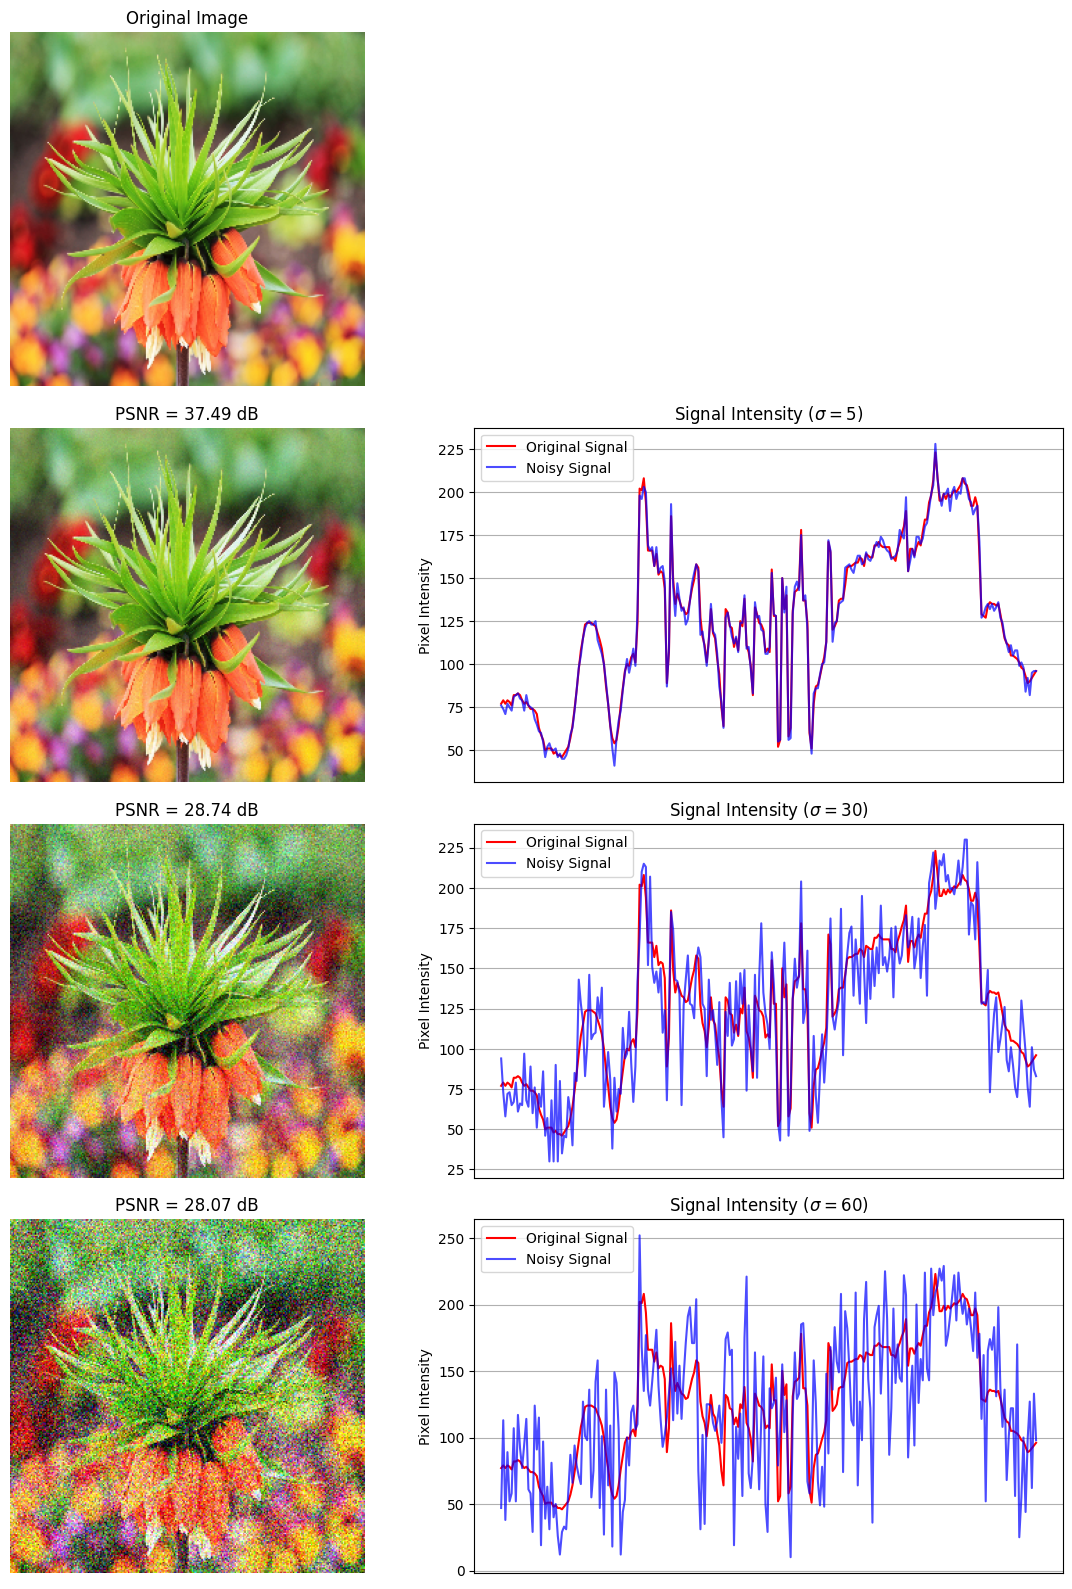
\includegraphics[width=0.6\textwidth]{figures/PSNR_plot.png}
    % \caption{Caption}
    \label{PSNR plot}
\end{figure*}


\textbf{Figure 7.1 Image with different PSNR.} Demonstrates noisy images with their corresponding PSNR values compared to the
original ones. \textbf{Left:} Original image and its noisy version. 
\textbf{Right:} Illustration of how strong noise signals have been added to the original image.
The color image is from the popular \href{https://data.vision.ee.ethz.ch/cvl/DIV2K/}{DIV2K} dataset.
\vspace{-12pt} 

\orangebox{Did you know that...}
{PSNR is not just for images; it can be applied to \textbf{video, audio, or even signal processing}. Anytime we want to
measure the quality of \textbf{reconstructed} signal compared to the \textbf{original}, PSNR could be considered.}

\vspace{-5pt} 

\textbf{Other related metrics}

\vspace{-5pt} 

Modern computer vision problems often focus on generating likely realistic images that are perceptually pleasing to humans,
rather than strictly matching the
target image pixel by pixel. Therefore, PSNR is typically used in conjunction with other modern metrics like Fréchet Inception
Distance (FID) or Inception Score (IS).



\chapter{NLP}


% ---------- Bilingual Evaluation Understudy ----------
\clearpage
\thispagestyle{nlpstyle}
\section{BLEU}
\subsection{Bilingual Evaluation Understudy}

BLEU is one of the earliest and most widely used metrics for evaluating machine translation and other
text generation tasks. It measures how similar a machine-generated text is to one or more human
reference translations by calculating the overlap of n-grams (contiguous sequences of words).

% equation
\begin{center}
    FORMULA GOES HERE
\end{center}

BLEU ranges from 0 to 1, where 1 indicates a perfect match with the reference.

\textbf{When to use BLEU?}

Use BLEU when evaluating machine translation, summarization, or text generation models where direct
word or phrase overlap with human-produced references is important.

\coloredboxes{
\item Correlates with human judgments at the corpus level. In its original study, BLEU showed strong
alignment with human evaluators.
\item Supports multiple references. Several human translations can be used, helping BLEU capture
natural variability.
\item To prevent models from producing unrealistically short outputs, BLEU introduces a
brevity penalty.
}
{
\item Insensitive to meaning. BLEU measures surface-level word overlap and does not account for
semantic equivalence.
\item Vulnerable to synonyms and paraphrasing. Valid alternative phrasings are not rewarded.
\item Sensitive to tokenization and normalization choices. BLEU scores can vary depending on how words
are segmented (e.g., handling of punctuation, casing, or subword units).
}

\clearpage

\thispagestyle{customstyle}

\orangebox{Did you know that...}
{BLEU was introduced in 2002 by Papineni et al. at IBM and was the first automatic metric to gain
wide acceptance in machine translation research.}


% ---------- Metric for Evaluation of Translation with Explicit ORdering ----------
\clearpage
\thispagestyle{nlpstyle}
\section{METEOR}
\subsection{Metric for Evaluation of Translation with Explicit ORdering}

METEOR (Metric for Evaluation of Translation with Explicit ORdering) is a machine translation
evaluation metric introduced as an improvement over BLEU. Unlike BLEU, which relies heavily on
exact n-gram matches, METEOR aligns candidate translations with reference translations using stemming,
synonyms, and paraphrases. 

% equation
\begin{center}
    FORMULA GOES HERE
\end{center}

It then computes a harmonic mean of unigram precision and recall, with
recall weighted higher to better capture adequacy. Finally, it introduces a fragmentation penalty to
account for word order, rewarding translations that are both accurate and fluent.

\textbf{When to use METEOR?}

It is especially valuable when translation adequacy (capturing meaning) is as important as fluency.
Because it incorporates linguistic resources such as stemming and synonyms, METEOR is useful for
low-resource or morphologically rich languages, where exact matches are too strict.

\coloredboxes{
\item Closer to human judgment. METEOR was shown to correlate better with human evaluations compared
to BLEU.
\item Flexible matching. Accounts for stemming, synonyms, and paraphrases, making it more tolerant
to variation in expression.
\item Balances adequacy and fluency. By combining precision, recall, and word order penalties,
it reflects both meaning preservation and readability.
}
{
\item Computationally heavy. Requires linguistic resources (stemming, synonym databases),
making it slower than purely statistical metrics.
\item Language dependence. Its quality depends on the availability and completeness of stemming
rules and synonym dictionaries for the target language.
}

\clearpage

\thispagestyle{customstyle}

\orangebox{Did you know that...}
{METEOR was developed at Carnegie Mellon University in 2005 as a direct response to BLEU’s shortcomings.}
\chapter{GenAI}


% ---------- Perplexity ----------
\clearpage
\thispagestyle{genaistyle}
\section{Perplexity}
\subsection{Perplexity}

% reference:
% https://aclanthology.org/2021.deelio-1.5.pdf
% https://kilthub.cmu.edu/articles/journal_contribution/Evaluation_Metrics_For_Language_Models/6605324/1?file=12095765
% https://huggingface.co/docs/transformers/perplexity
% https://brenocon.com/blog/2013/01/perplexity-as-branching-factor-as-shannon-diversity-index/

Perplexity is a widely used metric for evaluating language models. At its core, perplexity measures how well a probability distribution or model
predicts a sample. Mathematically, it is defined as the exponential of the average negative log-likelihood of the sequence. Intuitively, you can
think of it as the “average branching factor” — the number of equally likely choices the model considers at each step.

% equation
\begin{center}
    FORMULA GOES HERE
\end{center}

A lower perplexity indicates that the model assigns higher probabilities to the observed text, meaning it is less “surprised”.

\textbf{When to use Perplexity?}

Perplexity is most commonly used when evaluating language models during training or benchmarking. It helps track how well a model fits text data and
is especially useful for comparing models trained on the same dataset. However, perplexity is best suited for probabilistic next-token prediction
tasks and less reliable as a direct measure of end-user text quality.

\coloredboxes{
\item Simple and interpretable. Lower perplexity values generally mean better predictive performance.
\item Efficient for training evaluation. It provides a direct signal for model optimization without requiring human evaluation.
}
{
\item Models with low perplexity may still generate incoherent or unhelpful text.
\item Sensitive to tokenization and normalization choices.
\item Not well-defined for masked language models. Architectures like BERT predict missing tokens rather than generating sequences left-to-right,
making perplexity unsuitable for evaluating them.
}

\clearpage

\thispagestyle{customstyle}

\orangebox{Did you know that...}
{Perplexity is closely related to entropy in information theory. In fact, $Perplexity = 2^{H(P)}$
where \(H(P)\) is the entropy. This means that perplexity can be seen as the effective 
number of equally likely words the model is choosing from at each step!}

% ---------- BERTScore ----------
\clearpage
\thispagestyle{genaistyle}
\section{BERTScore}
\subsection{BERTScore}

% reference:
% https://arxiv.org/pdf/1904.09675
% https://wiki.math.uwaterloo.ca/statwiki/index.php?title=BERTScore:_Evaluating_Text_Generation_with_BERT

BERTScore is a metric for evaluating text generation that leverages contextual embeddings from pre-trained language models like BERT.
Instead of relying solely on surface-level n-gram overlap (as in BLEU or ROUGE), BERTScore computes similarity by aligning tokens from the
candidate and reference sentences in embedding space.

% equation
\begin{center}
    FORMULA GOES HERE
\end{center}

Mathematically, for each token in a candidate sentence, BERTScore finds its most similar token in the reference sentence (and vice versa)
using cosine similarity. Precision, recall, and F1 are then aggregated over all pairs, yielding a semantic-oriented score that correlates
strongly with human judgments.

\textbf{When to use the BERTScore?}

Use BERTScore when evaluating tasks where semantic similarity matters more than exact wording, such as machine translation, summarization, or
dialogue generation. It is especially useful when generated text can be phrased differently from references but still convey the same meaning.

\coloredboxes{
\item Context-aware. Uses deep contextual embeddings, capturing meaning beyond surface word matches
\item Better correlation with humans. Empirical studies show BERTScore aligns more closely with human evaluation than BLEU or ROUGE.
}
{
\item Computationally heavy. Requires embedding extraction with large pre-trained models, making it slower than n-gram metrics.
\item Model dependence. Performance varies depending on which pre-trained model (e.g., BERT, RoBERTa, multilingual-BERT) is used.
\item Bias inheritance. Any biases in the underlying language model embeddings can influence the scores.
}

\clearpage

\thispagestyle{customstyle}

\orangebox{Did you know that...}
{The original BERTScore paper included a picture of Bert from Sesame Street paying homage to the model’s namesake and adding a playful touch to an
otherwise technical paper.}
\include{9-probabilistic}
\chapter{Bias \& Fairness}


% ---------- Demographic Parity ----------
\clearpage
\thispagestyle{biasfairnesstyle}
\section{Demographic Parity}
\subsection{Demographic Parity}

% reference:
% https://developers.google.com/machine-learning/crash-course/fairness/demographic-parity
% https://afraenkel.github.io/fairness-book/content/05-parity-measures.html#demographic-parity
% https://fairmlbook.org/classification.html

Demographic Parity (also known as Statistical Parity) is one of the most widely cited fairness metrics in machine learning.
It requires that the decision of a model be independent of a protected attribute (such as gender, race, or age). In other words,
the probability of receiving a positive prediction should be the same across groups, regardless of whether the prediction is correct.

% Formula
\begin{center}
    % P(Y^=1∣A=a)=P(Y^=1∣A=b)∀a,b
    FORMULA GOES HERE
\end{center}

A model satisfies demographic parity if members of different demographic groups are selected at equal rates. For example, in a loan approval
system, demographic parity would mean that the proportion of approved applications is the same across groups, independent of creditworthiness.

\textbf{When to use Demographic Parity?}

Use demographic parity when the fairness objective is equal treatment across groups in terms of outcomes, even if this comes at the cost
of predictive accuracy. It is often applied in contexts such as hiring, lending, or college admissions, where ensuring equal access is a
primary concern.

\coloredboxes{
\item Simple to compute and easy to explain to non-technical stakeholders.
\item Guarantees equal selection rates across groups, supporting inclusion.
}
{
\item It only looks at whether groups get the same share of positive outcomes, but not at whether those predictions are actually correct.
\item Can reduce overall model accuracy if the underlying distributions differ.
}

\clearpage

\thispagestyle{customstyle}

\orangebox{Did you know that...}
{Demographic parity goes by several other names in the literature, often referred to as statistical parity, group fairness, or even
independence criterion. Different research communities picked different terms, but they all describe the same idea.}


% ---------- Equality of Opportunity ----------
\clearpage
\thispagestyle{biasfairnesstyle}
\section{Equality of Opportunity}
\subsection{Equality of Opportunity}

Equality of Opportunity is a fairness metric that focuses on ensuring that individuals who truly belong to the positive class
(e.g., qualified applicants) have an equal chance of being correctly identified across different demographic groups.
Formally, the metric requires that the True Positive Rate (TPR) be equal across groups.

% Formula
\begin{center}
    % P(Y^=1∣Y=1,A=a)=P(Y^=1∣Y=1,A=b)
    FORMULA GOES HERE
\end{center}

In other words, if two people are equally qualified, their chance of being recognized as such by the model should not depend on their
demographic group.

\textbf{When to use Equality of Opportunity?}

This metric is particularly useful in high-stakes scenarios where false negatives carry large consequences, such as university admissions,
medical diagnoses, or loan approvals. It ensures that qualified individuals are treated equally, regardless of group membership.

\coloredboxes{
\item Ensures qualified individuals have equal chances across groups, even if overall acceptance rates differ.
\item Models can vary in their ratio of positive to negative predictions across groups, as long as the true positives are treated fairly.
\item Can be more aligned with fairness in practical scenarios, where ensuring equal opportunity for qualified candidates
is more meaningful than enforcing equal acceptance rates.
}
{
\item Only applies when there is a clearly preferred label (e.g., “qualified”), limiting its use to such contexts.
\item Does not guarantee fairness for the negative class, unlike metrics such as Equalized Odds.
\item Requires demographic group labels to compare outcomes. If group membership is unavailable, the metric cannot be applied.
}

\clearpage

\thispagestyle{customstyle}

\orangebox{Did you know that...}
{Equality of Opportunity was popularized in the 2016 paper “Equality of Opportunity in Supervised Learning” by Hardt, Price, and Srebro. 
In that paper, they introduced both Equality of Opportunity and its stricter sibling, Equalized Odds. The terms have since become standard
in the fairness in ML literature.}

% ---------- Equality of Odds ----------
\clearpage
\thispagestyle{biasfairnesstyle}
\section{Equality of Odds}
\subsection{Equality of Odds}

% resources:
% https://arxiv.org/pdf/1610.02413
% https://mlu-explain.github.io/equality-of-odds/

Equality of Odds is a fairness metric that requires a model to have equal true positive rates (TPR) and equal false positive rates (FPR)
across different demographic groups. In other words, the model should be equally good at identifying positives and equally bad at making mistakes,
no matter which group an individual belongs to.

% Formula
\begin{center}
    % P(Y^=1∣Y=y,A=a)=P(Y^=1∣Y=y,A=b)∀y∈{0,1},a,b∈A
    FORMULA GOES HERE
\end{center}

Equalized Odds is stricter than Equality of Opportunity, which only enforces equality on the true positive rate. If we relax the Equalized Odds
condition to focus only on the case where $Y = 1$, we obtain the Equality of Opportunity formula.

\textbf{When to use Equality of Odds?}

Use Equality of Odds when both types of classification errors, false positives and false negatives, carry important consequences.
For example, in loan approvals, we want to ensure that different groups are not only equally likely to receive a loan when they are
truly creditworthy, but also equally likely to be mistakenly given a loan when they are not.

\coloredboxes{
\item Captures fairness across both positive and negative outcomes.
\item More comprehensive than Equality of Opportunity, which only balances true positive rates.
}
{
\item May be difficult or impossible to satisfy perfectly, especially when the distribution of labels differ across groups.
\item Enforcing Equality of Odds can reduce overall model accuracy, creating a trade-off between fairness and performance.
}

\clearpage

\thispagestyle{customstyle}

\orangebox{Did you know that...}
{Equality of Odds was popularized in the 2016 paper “Equality of Opportunity in Supervised Learning” by Hardt, Price, and Srebro. 
In that paper, they introduced both Equality of Odds and its less stricter sibling, Equality Opportunity. The terms have since become standard
in the fairness in ML literature.}

% For second page we can follow The ROC Curves example of this resource: https://mlu-explain.github.io/equality-of-odds/
\chapter{Bussiness}


% ---------- Bussiness Sample Metric ----------
\clearpage
\thispagestyle{businessstyle}
\section{Bussiness Sample Metric}
\subsection{Bussiness Sample Metric}

% ---------- CR ----------
\clearpage
\thispagestyle{businessstyle}

\section{CR}

\subsection{Conversion Rate}
In machine learning, Conversion Rate is the percentage of users who complete a desired action after being targeted by a model's recommendations or predictions.
For instance, in e-commerce conversion rate measures the percentage of users who purchase after receiving product recommendations from a machine learning model.

% equation
\begin{center}
    \tikz{
        \node[inner sep=2pt, font=\large] (a) {
            {
                $\displaystyle
                 Conversion \, Rate =\frac{Number \, of \,Conversions}{Number \, of \, Visits}\times100
                $
            }
        };
    }
\end{center}

\vspace{-10pt}

A high conversion rate indicates that the model successfully identifies and engages relevant users, leading to effective recommendations and increased sales.

\textbf{When to use Conversion Rate?}

Use conversion rate to evaluate marketing effectiveness, website performance, and user experience optimization, especially during campaigns, A/B testing, and product launches.

\coloredboxes{  % Ensure that this command is defined in your preamble
\item Provides a direct, measurable way to assess the effectiveness of machine learning models, marketing campaigns, or recommendation systems.
\item Versatile across various domains, including e-commerce, online advertising, and product recommendations.
}
{
\item Ignores positive user engagement that doesn’t lead to immediate conversions.
\item Optimizing for conversion rate can sometimes favor short-term wins over long-term user experience.
}

\textbf{Other related metrics}

Other related metrics to Conversion Rate include Bounce Rate and Return on Investment (ROI).


\end{document}